\documentclass{article}
\usepackage[utf8]{inputenc}
\usepackage{circuitikz}
\usepackage{amsmath}
\usepackage{fullpage}
\usepackage{hyperref}
\usepackage{graphicx} 
\usepackage{float}
\usepackage{booktabs}
\usepackage{multirow}
\usepackage{amsfonts}
\usetikzlibrary{arrows}
\usetikzlibrary{shapes.geometric}
\usepackage{siunitx}
\usepackage{natbib}
\usepackage{subcaption}
\usepackage{pgfplots}
\pgfplotsset{compat=1.13}
\usepgfplotslibrary{units}
\usepackage{array}
\usepackage{subcaption}

% http://www.mathworks.com/matlabcentral/fileexchange/8015-m-code-latex-package
\usepackage{mcode}

\usepackage{siunitx} % gotta get those units

\usepackage{booktabs} % do you like nice tables? I like nice tables
\usepackage{array}    % do crazy table stuff (center align those paragraphs!)

\setlength{\heavyrulewidth}{1.5pt} % table setup stuff
\setlength{\abovetopsep}{4pt}      % these tables are going to look so nice

%Making a new function for somewhat more beautiful abs() functions
\newcommand\abs[1]{\left|#1\right|}
%Package for roman number 
\makeatletter
\newcommand*{\rom}[1]{\expandafter\@slowromancap\romannumeral #1@}


\title{EPO-1 D2 Speaker \rom{2}}
\author{Arthur Admiraal (4545532)\\
Olivier Dingeldein (4576012)\\
Aschraf Gardouh (4579941)\\
Tarik Benaich*(4609980)\\
Koen de Bruijn (4587200)\\
Avinash Kalloe*(4574427)\\
Stan Kamiński  (4534166)\\
Jasper Rietveld*(4581881)\\
Lynrick Wix (4534654)\\
Baris Yakali* (4577078)}
\date{November 2016}

\begin{document}
\begin{titlepage}
  \maketitle
\end{titlepage}
\tableofcontents\newpage

\section{Introduction} 
Designing a speaker filter requires data about the frequency response of the loudspeaker, so that the filters can correct for it and provide a flatter audio response. Our three-way speaker system consists of three separate speaker elements, which are called `woofer', `mid-range', and `tweeter' from hereon, in order of increasing frequency. The aim of this work is twofold:
\begin{itemize}
  \item Establish and dimension electric equivalent circuits of each speaker element in such a way that the resulting impedance corresponds as much as possible to the measured impedance.
  \item Find the acoustic transfer of each speaker element, containing both magnitude and phase components.
\end{itemize} 
These results should be valid over the complete frequency range of this system, ranging from $20\si{\hertz}$ until $20\si{\kilo\hertz}$.\\ 
\newline
The measurements that will be made can be used for the filter design: The frequency response measurements can then be used for choosing the right cut-off frequency and the impedance model can be used to design zobel networks inside the filter.\\ 
\newline
In the following sections, you will first present an overview of the equivalent model including component dimensioning. Subsequently, the simulation and measured results will be discussed. Furthermore, the measurement setup for both impedance and short distance acoustic measurements will be taken under consideration. We finish with the conclusion and recommendations.


\begin{figure}[ht]
  \centering
  \begin{circuitikz}
    \draw (0,0) to[amp, o-*] (2,0)
      -- (2,2)
      to[highpass] (4,2)
      to[twoport] (6,2);
    \draw (2,0) to[bandpass] (4,0)
      to[twoport] (6,0);
    \draw (2,0) -- (2,-2)
      to[lowpass] (4,-2)
      to[twoport] (6,-2);
    
    % power supply
    \draw[-latex] (1,-1) -- (1,-0.26);
    \node[draw,thick,minimum width=1cm,minimum height=1cm] at (1,-1.5) {supply};
    
    % speakers - a hack, but working
    % high
    \node[draw,thick,right,minimum width=0.3cm,minimum height=0.8cm] at (6,2) {};
    \node[rotate=90,trapezium,draw,thick,below,trapezium angle=55,minimum width=0.7cm,minimum height=0.5cm] at (6.3,2) {};
    \node[right] at (7,2) {tweeter};
    
    % mid
    \node[draw,thick,right,minimum width=0.3cm,minimum height=0.8cm] at (6,0) {};
    \node[rotate=90,trapezium,draw,thick,below,trapezium angle=55,minimum width=0.7cm,minimum height=0.5cm] at (6.3,0) {};
    \node[right] at (7,0) {mid-range};
    
    % low
    \node[draw,thick,right,minimum width=0.3cm,minimum height=0.8cm] at (6,-2) {};
    \node[rotate=90,trapezium,draw,thick,below,trapezium angle=55,minimum width=0.7cm,minimum height=0.5cm] at (6.3,-2) {};
    \node[right] at (7,-2) {woofer}; 
    
    \draw[gray, dashed] (2.3,2.7) rectangle (3.7,-2.7);
    \draw[gray, dashed] (4.3,2.7) rectangle (5.7,-2.7);
    
    \draw[gray, dashed] (0.2,-2.1) rectangle (1.8,-0.9);
    \node[left, gray] at (0.2,-1.5) {Power Supply};
    
    \node[left]        at (0,0)    {line in};
    \node[above, gray] at (3,2.7)  {three-way divider};
    \node[below, gray] at (5,-2.7) {linearisation};
  \end{circuitikz}
  \label{fig:blockdiagram}
  \caption{Block diagram of the system with the filters, power supply and the power amplifier}
\end{figure}

\newpage\section{Loudspeaker Analysis}
\subsection{Circuit Schematics}\label{sec:circuitschematics}

\begin{figure}[ht!]
  \centering
  \begin{circuitikz}
    \draw (0,5) to[short, o-] (2,5)
      to[R, l=$R_e$] (2,3.5)
      to[L, l=$L_e$, -*] (2,2)
      -- (1,2)
      to[R, l_=$R_p$] (1,0.5)
      to[short, -*] (2,0.5)
      --(2,0) to[short, -o] (0,0);
    \draw (2,2) to[C, l=$C_p$] (2,0.5);
    \draw (2,2) -- (3.3,2)
      to[L, l=$L_p$] (3.3,0.5)
      -- (2,0.5);
  \end{circuitikz}
  \caption{Equivalent circuit of a speaker element}
  \label{fig:eqcircuit}
\end{figure}

An equivalent circuit of a speaker element is shown in figure \ref{fig:eqcircuit}. $R_e$ is the DC resistance of the voice coil, $L_e$ the self-inductance of the voice coil and the resonant RLC network consisting of the inductor $L_p$, the capacitor $C_p$ and the resistor $R_p$ models influence the resonant properties of the mechanical system (\cite{studentmanual}).

\subsection{Equations for model 1}
With the equivalent circuit model in hand, we can dimension it for the various speaker elements.

The value of $R_e$ is equal to the DC resistance of the speaker, as the impedances of the coils are $0\si{\ohm}$ at DC. This can simply be measured using a multimeter.

The other values can be derived from impedance measurements. In appendix \ref{app:deriv} we derive several formulas to calculate the component values from characteristics of the impedance measurements and previously calculated values:
\begin{align*}
  R_p &= \abs{Z_{ls}(\omega_0)} - R_e                   \tag{\ref{eq:rp}}\\
  C_p &= \frac{1}{B_w \cdot R_p}                        \tag{\ref{eq:cp}}\\
  L_p &= \frac{1}{\omega_0^2 \cdot C_p}                 \tag{\ref{eq:lp}}\\
  L_e            &= \sqrt{\frac{\abs{Z_{ls}}^2 - R_e^2}{\omega^2}}\label{eq:le}
\end{align*}

By using these formulas, the values for the model given in section \ref{sec:circuitschematics} can be computed. As an example, the calculations that were done to compute the component values for the bass speaker will be described.
\newpage
The values of $R_e$ had been measured to be $4.00 \  \Omega$.

Then, the values for the values $\omega_0$ and the value $R_p$ are obtained from the impedance measurement results. For the bass speakers, the results were as follows:

\begin{figure}[ht]
  \centering
  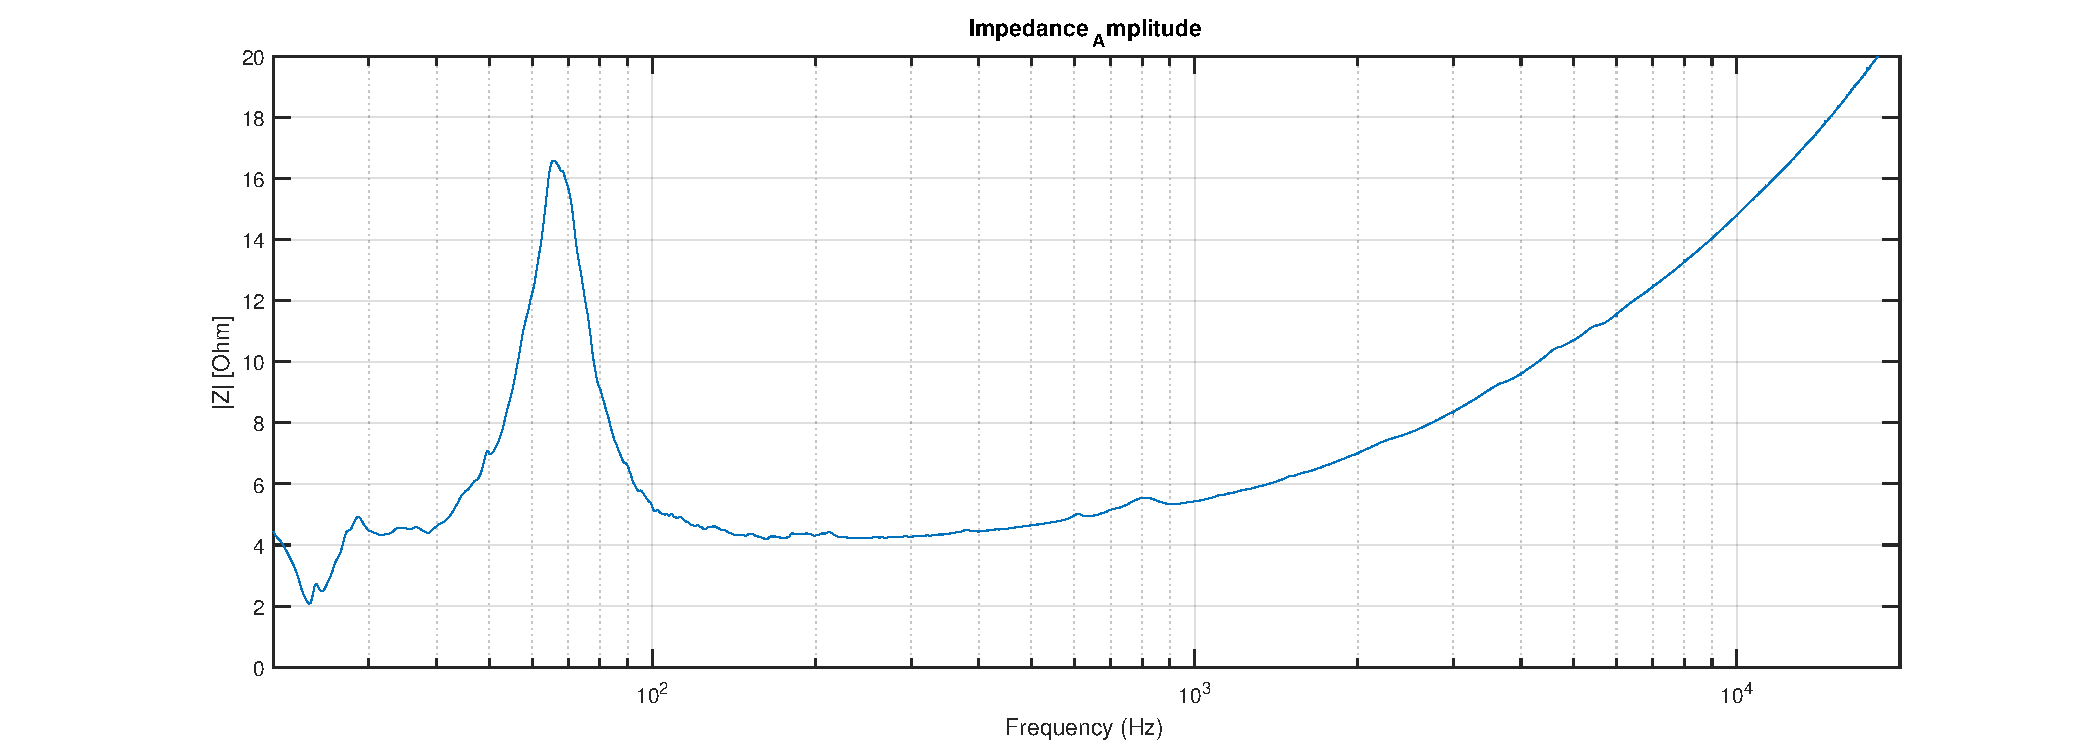
\includegraphics[height=0.2\paperheight]{Figures/Bass_Impedance_Measurements}%
  \label{fig:Bass_Impedance_Measurements}
  \caption{Impedance measurements for the bass speakers}
\end{figure}

By using MatLabs 'Data Cursor' tool, it can be read that the peak of the graph lies at $f = 65.73 \ Hz$, $\abs{Z} = 16.58 \ \Omega$. To get $\omega_0$ we then multiply the frequency by $2\pi$, thus obtaining:
\newline
$$\omega_0 = 2\pi f \approx 413.0 \ rad/s$$
\newline
The value of $R_p$ is obtained with the formula $R_p = \abs{Z_{ls}(\omega_0)} - R_e$. One then obtains: 
\newline
$$R_p = 16.58 - 4.00 = 12.58\ \Omega$$
\newline
To obtain the bandwidth, the Data Cursor is used to find the frequencies $\omega_1$ and $\omega_2$ at which the impedance is as close as possible to $R_e + R_p \frac{1}{\sqrt{2}} = 4.00 + 12.58 \frac{1}{\sqrt{2}} \approx 12.90$. One then finds:
\newline
$$\omega_1 = 2\pi * 60.97 \approx 383.1\ rad/s$$
$$\omega_2 = 2\pi * 73.79 \approx 463.6\ rad/s$$. 
\newline
the bandwidth can then be calculated by calculating the difference between $\omega_1$ and $\omega_2$: 
\newline
$$B_w = \omega_2 - \omega_1 = 463.6 - 383.1 = 80.50 $$
\newline 
With the bandwidth the component values of $C_p$ and $L_p$ Can be calculated. for $C_p$:
\newline
  $$C_p = \frac{1}{B_w \cdot R_p} = \frac{1}{80.50 \cdot 12.58} \approx 987.5\ \si{\micro\farad}$$
\newline
Then for $L_p$:
\newline
  $$L_p = \frac{1}{\omega_0^2 \cdot C_p} = \frac{1}{413.0^2 \cdot 987.5\cdot10^{-6}} = 5940\ \si{\micro\henry}$$
\newline
To find $L_e$, a point at a high frequency is read from the data. For this, $f = 10\ \si{\kilo\hertz}$ is chosen. one then finds $\abs{Z_Ls} = 14.80\ \Omega$. One can then calculate $L_e$:
$$L_e = \sqrt{\frac{\abs{Z_{ls}}^2 - R_e^2}{\omega^2}} = \sqrt{\frac{\abs{14.80}^2 - 4.00^2}{(2\pi\cdot10\si{\kilo})^2}} \approx 227\ \si{\micro\henry}$$
\newline
The calculations for all the speakers resulted in the values found in table \ref{tab:componentvalues}.

\begin{table}[ht] % moar tables!!!!11!!!1!
  \centering
  \begin{tabular}{p{1.3cm} >{\centering\arraybackslash}p{1.3cm} >{\centering\arraybackslash}p{1.3cm} >{\centering\arraybackslash}p{1.3cm}}
    \toprule
     & \textbf{low} & \textbf{mid} & \textbf{high} \\
    \midrule
    $R_e\ (\si{\ohm})$          & 4.00 & 3.70  & 3.90 \\
    $L_e\ (\si{\micro\henry})$  & 227  & 220   & 84.5 \\
    $R_p\ (\si{\ohm})$          & 12.6 & 6.88  & 4.71 \\
    $C_p\ (\si{\micro\farad})$  & 987  & 1560  & 75.1 \\
    $L_p\ (\si{\micro\henry})$  & 5940 & 2330  & 512  \\
    \bottomrule
  \end{tabular}
  \caption{Various component values.}
  \label{tab:componentvalues}
\end{table}

\section{Simulations}
The component values that were computed in the previous section can be used to create a simulation of the model. This model can be derived by using nodal analysis, due to the components being parallel to each other.
\newline
To do this, the values in the circuit are first converted from the frequency domain to the time domain. In the frequency domain, the impedance of a Resistor, an inductor, and a capacitor are given by:

$$ Z_{Resitor} = R $$
$$ Z_{Inductor} =  j \omega L $$
$$ Z_{Capacitor} = \frac{1}{j \omega C} $$
\newline 
The Impedances of the model can then be added and calculated like resistances. This results in the following equations for the used model:

$$ Z = Z_{L_e} + Z_{R_e} + Z_{R_p}||Z_{L_p}||Z_{C_p} $$

$$ Z = Z_{L_e} + Z_{R_e} + \frac{1}{ \frac{1}{Z_{R_p}}  + \frac{1}{Z_{L_p}} + \frac{1}{Z_{C_p}}} $$
If the impedances of the different components are then filled in to get an equation for the inductance of the circuit based as a function of the angular frequency $\omega$. The impedance of the electrical model is then given by:

$$Z(\omega) = R_e + j \cdot \omega \cdot L_e + \frac{1}{ \frac{1}{R_p} + j \cdot \omega \cdot C_p + \frac{1}{j \cdot \omega \cdot L_p} }$$
\newline
This model is then used to calculate the impedance of the model at different input frequencies in a MatLab script. The resulting values of the impedance is then drawn into a graph. since the voltage source in the frequency domain may be complex, the abstract value is calculated to create the graph. The function thus becomes:
\newline
$$\abs{Z(\omega)} = \abs{R_e + j \cdot \omega \cdot L_e + \frac{1}{ \frac{1}{R_p} + j \cdot \omega \cdot C_p + \frac{1}{j \cdot \omega \cdot L_p} }}$$
\newline
The final MatLab script that has been created to model the impedance and graph the results can be found in appendix 2.
\newline
The graphs that were produced using the MatLab script and the calculated values are located in appendix C.1. For the mid, the graph is also found below here.

\begin{figure}[H]
  \centering
  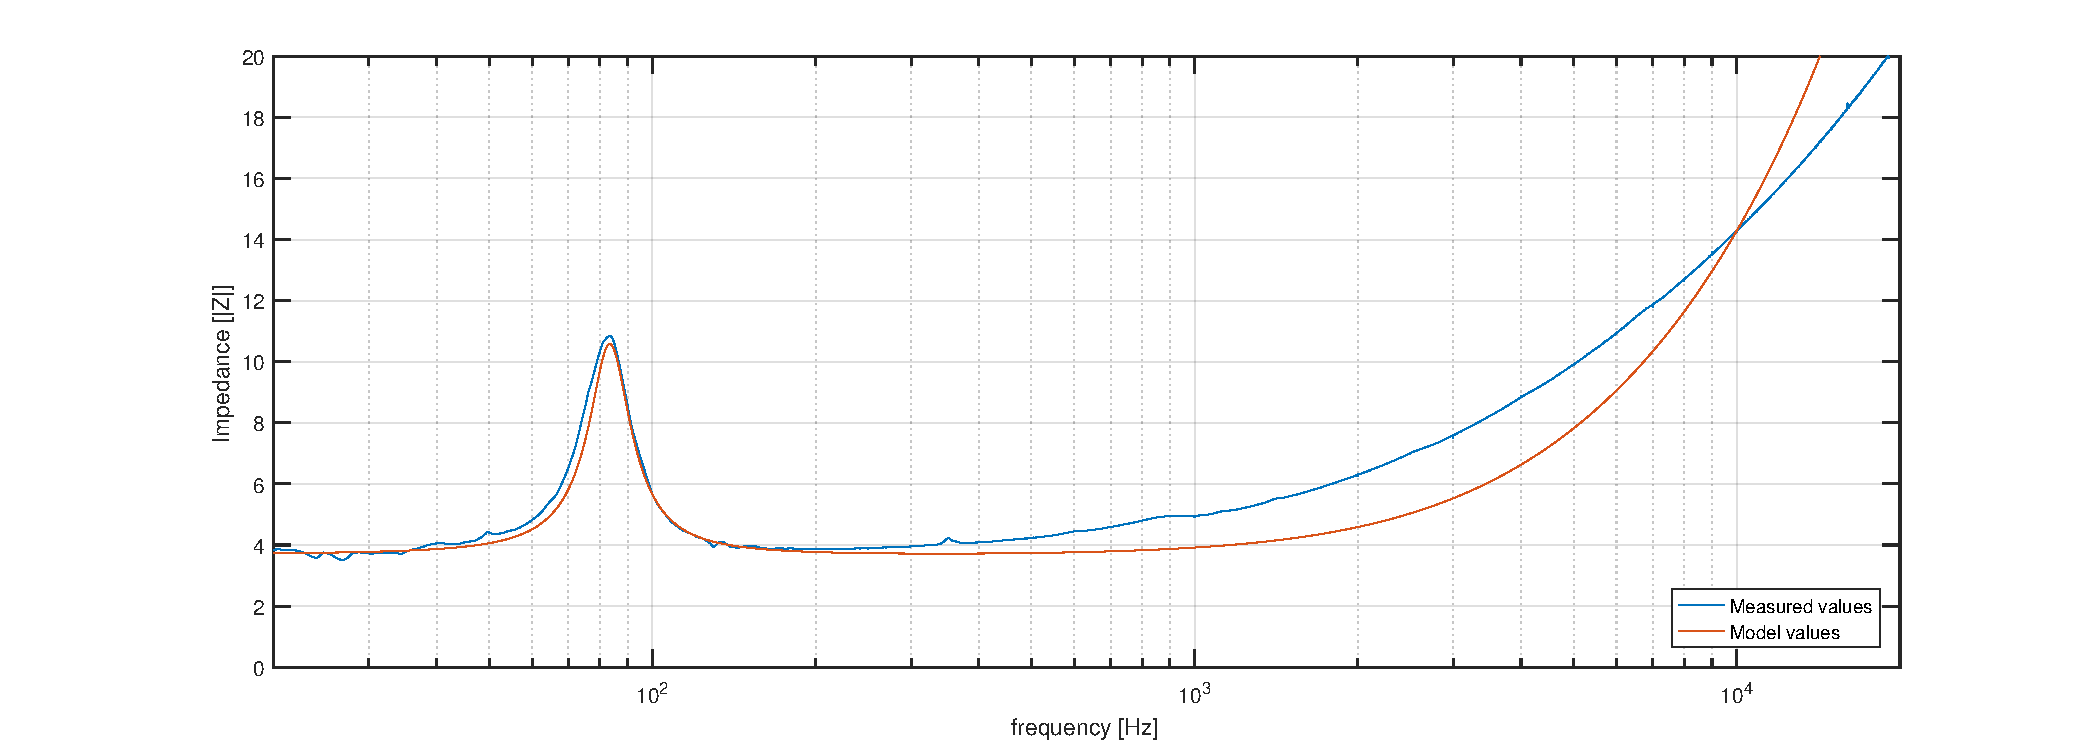
\includegraphics[height=0.2\paperheight]{Figures/Mid_Impedance_Model_Calculated.pdf}%
  \label{fig:Mid_Impedance_Model_Calculated_inText}
  \caption{Calculated Impedance model for the mid speaker with the measurements for comparison}
\end{figure}

As one can see, the models are reasonably accurate around the resonance peaks. However, at values above the resonance peak, the model turns out to have a significantly different impedance. This difference in impedance may have several causes. Possibly our model is not entirely perfect. Multiple factors may not have been taken into account. These factors may include the acoustics of the speaker case or the 
\newline 
\newline 
From this one can conclude that the model that was used may not represent the actual speakers perfectly for the frequencies well above the resonance peak. In this area, the impedance of our model is caused primarily by the impedance of the self inductance of the voice coil L\textsubscript{e} and the resistance R\textsubscript{e}: 
$$\abs{Z_{ls}} = \abs{R_e + j \omega L_e}$$
\newline
this function increases linearly. However, the measured impedance seems to be not entirely linear as it curls up at higher frequencies. This formula has been used to calculate L\textsubscript{e}. The rewritten equation that has been used for this is as follows:
\newline
$$L_e =\sqrt[]{\frac{R_e^2 - Z_{ls} ^2}{\omega^2}}$$
\newline
To obtain Z\textsubscript{ls} and $\omega$ a point in the graph of the impedance measurements was chosen. However, because the measured impedance is not linear, if one chooses different points to calculate L\textsubscript{e}, the obtained graph will differ. This means that the model could be changed to be more accurate by choosing various points in the measurements.
\newline
\newline
In order to find the value of L\textsubscript{e}, that gave results that matched as closely to the measured impedance as possible, a specific MatLab function called 'function fit' was used. This function tests different values for input variables in a function in order to make it match as closely as possible to input data. In this case, the input variables are the component values, the function is the function used to calculate the impedance and the input data are the impedance measurements.
\newline
\newline
The MatLab script that has been created and used for the function fit can be found in appendix B.2.
\newline
\newline
By efficiently choosing the starting points and bounds of the input variables and by limiting the function fit to specific parts of the input data,
the efficiency of the function fit can be increased significantly.
\newline
\newline

By using the function fit, the following values have been found:
\newline
\begin{table}[ht] % I made another table :D
  \centering
  \begin{tabular}{p{1.3cm} >{\centering\arraybackslash}p{1.3cm} >{\centering\arraybackslash}p{1.3cm} >{\centering\arraybackslash}p{1.3cm}}
    \toprule
     & \textbf{low} & \textbf{mid} & \textbf{high} \\
    \midrule
    $R_e\ (\si{\ohm})$          & 4.00 & 3.70  & 4.30 \\ 
    $L_e\ (\si{\micro\henry})$  & 922  & 437   & 74.2 \\
    $R_p\ (\si{\ohm})$          & 12.6 & 6.88  & 4.31 \\
    $C_p\ (\si{\micro\farad})$  & 808  & 1513  & 71.6 \\ 
    $L_p\ (\si{\micro\henry})$  & 6844 & 2456  & 519  \\
    \bottomrule
  \end{tabular}
  \caption{Component values derived from function fit.}
  \label{tab:componentvaluesfit}
\end{table}
\newline
If these values are then used in the modelling script, one gets new graphs that should resemble the measurements more. For the mid the results can be seen in the figure below. The graphs that have been found with these values are located in appendix C.2 

\begin{figure}[ht]
  \centering
  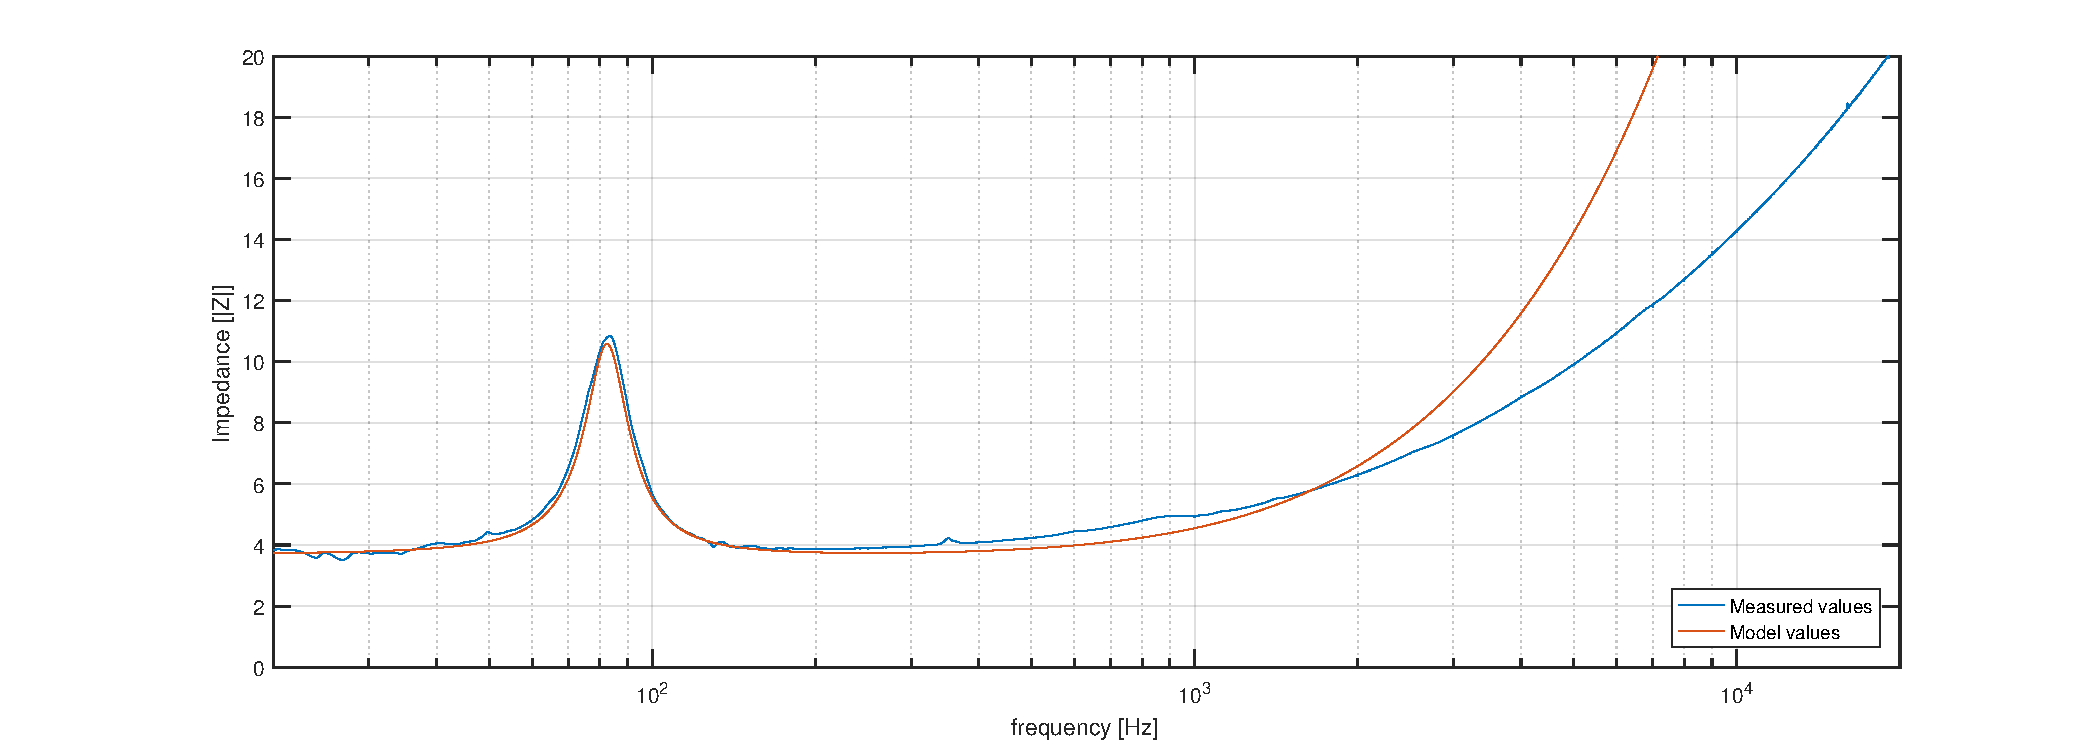
\includegraphics[height=0.2\paperheight]{Figures/Mid_Impedance_Model_Fitted.pdf}%
  \label{fig:Bass_Impedance_Model_Fitted_inText}
  \caption{Fitted Impedance model for the mid speaker with the measurements for comparison}
\end{figure}

In order to determine the relative size of the deviation of the model before and after the fit, another MatLab program has to be used and created. By using this script the relative deviation of a function in respect to input data can be graphed as a function of the frequency and the average relative deviation can be calculated. By using this program, the increase in accuracy of the new model can be determined. The resulting graph for the mid can be found in the figure below. The other graphs are to be found in appendix C.3.

\begin{figure}[H]
  \centering
  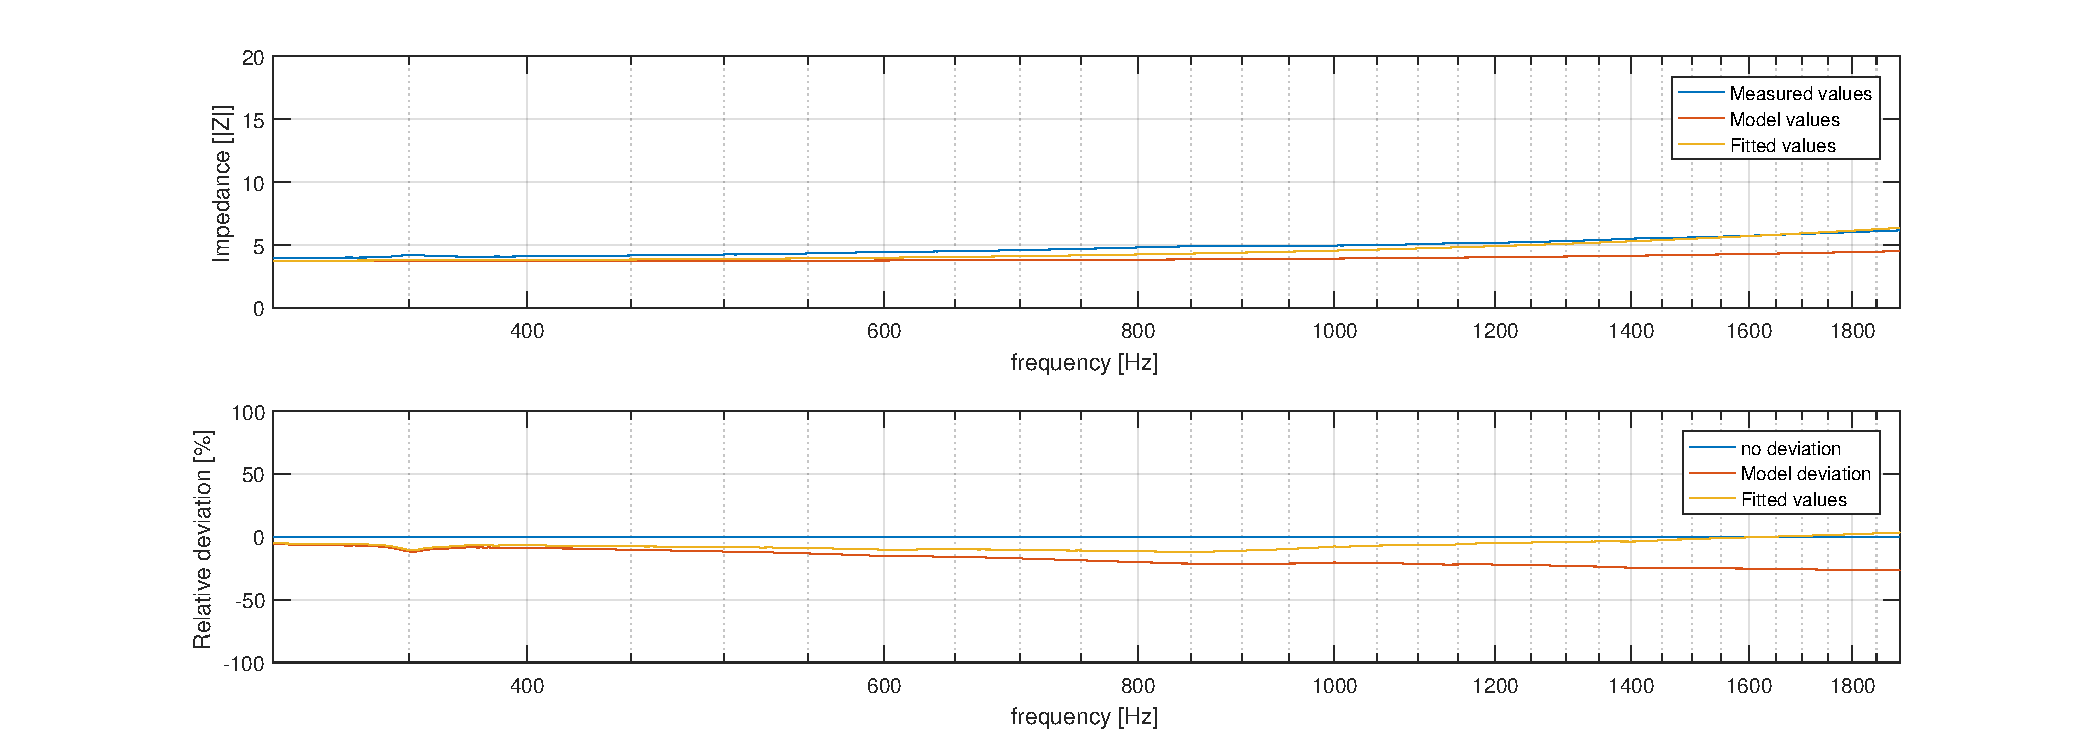
\includegraphics[height=0.15\paperheight]{Figures/Relative_Deviation_Mid_Impedance_Models.pdf}%
  \label{fig:Relative_Deviation_Mid_Impedance_Models_inText}
  \caption{Relative deviation graphs for the mid speaker models on it's frequency range}
\end{figure}

We can therefore conclude that the models have indeed been improved. Hence, we use the values of the fitted curves instead of the calculated values. 
\newline
\newline
The scripts used for the calculation of the relative deviation can be found in appendix B.3.


\section{Measurements}
\subsection{Short Distance Acoustic Measurements}
\subsubsection{Equipment}
For the measurements of the short distance acoustic measurements, we followed the guidelines of the Studentmanual. First we obtained all the necessary items, which include: a connector box, buffer amplifier, microphone amplifier, the microphone itself, the oscilloscope, two jack-jack cables, several banana-plug to banana-plug cables, and a 2 x banana-plug to BNC cable.

\subsubsection{Setting-up}
The first step was to connect the line in and out to the connector box, which had been set to "Freq. Overdracht" for this particular measurement. This was very simple, as the line out of the PC had to be connected to the line out of the connector box. The only thing we noticed was that the back of the computer could only be used for line out. V\textsubscript{out} had to be connected to the buffer amplifier with the 2 x banana-plug to BNC cable. The second banana-plug was used to connect the ground, to ensure a common ground between all the components. The output of the buffer amplifier was coupled with the individual speaker elements, as well as the oscilloscope. These elements included: the tweeter, mid-range, woofer, and the woofers combined, because we had two woofers available. On the other side, the microphone was coupled with the microphone amplifier, which had to be made in assignment 4. This amplifier was then linked to the connector box. Now everything was set, all that needed to be done was power both the amplifiers and make sure that every peripheral had a common ground. 
\subsubsection{Measurement Procedure}
After the whole system was connected and ready, the next step was to fix everything in the software department. The file "LS-Measure" was opened in MatLab and the option "Overdracht-Meting" had been chosen. The only selections which had to be changed were the F\textsubscript{min}, F\textsubscript{max}, and ML-generator length. The minimum and maximum value were set at 20Hz and 20kHz respectively. The value of the ML-generator length was changed to 18, as this was the best value which was both accurate did not take too long to load.
\newline
Now it was time to power everything up. this meant, connected both the amplifiers to a DC voltage power supply and turn the oscilloscope on. The first trial could now be done, after one small adjustment. The oscilloscope had to show a peak-to-peak voltage of 2 to 3 volts. Therefore, with the first trial the output voltage was adjusted until the desired values were reached. Then finally it was time to start the actual measurements. The tweeter was up first, as it would have been appropriate to start high and work our way down to the lows.
\newline
All the speaker components were measured in the same way. The microphone was set to distance of 2cm from the cone and the program was started. After sometime of random noise, the speaker was still and the graph showed up on the screen. This was done 4 times to ensure that the graph which showed up was as accurate as possible. The graph was then saved and shared with the rest of the group for their convenience. This was done for all the four components. However, there was one extra measurement. At the end of all the measurements, the two woofers were connected in parallel and the measured. The microphone also had to change its position, this position was between the two woofers. The relevance of this measurement was to see how the phase shift would change.


\begin{figure} [H]
\subcaptionbox{Frequency response of the mid.  \label{fig:Mid_Response_JBT}}{%
  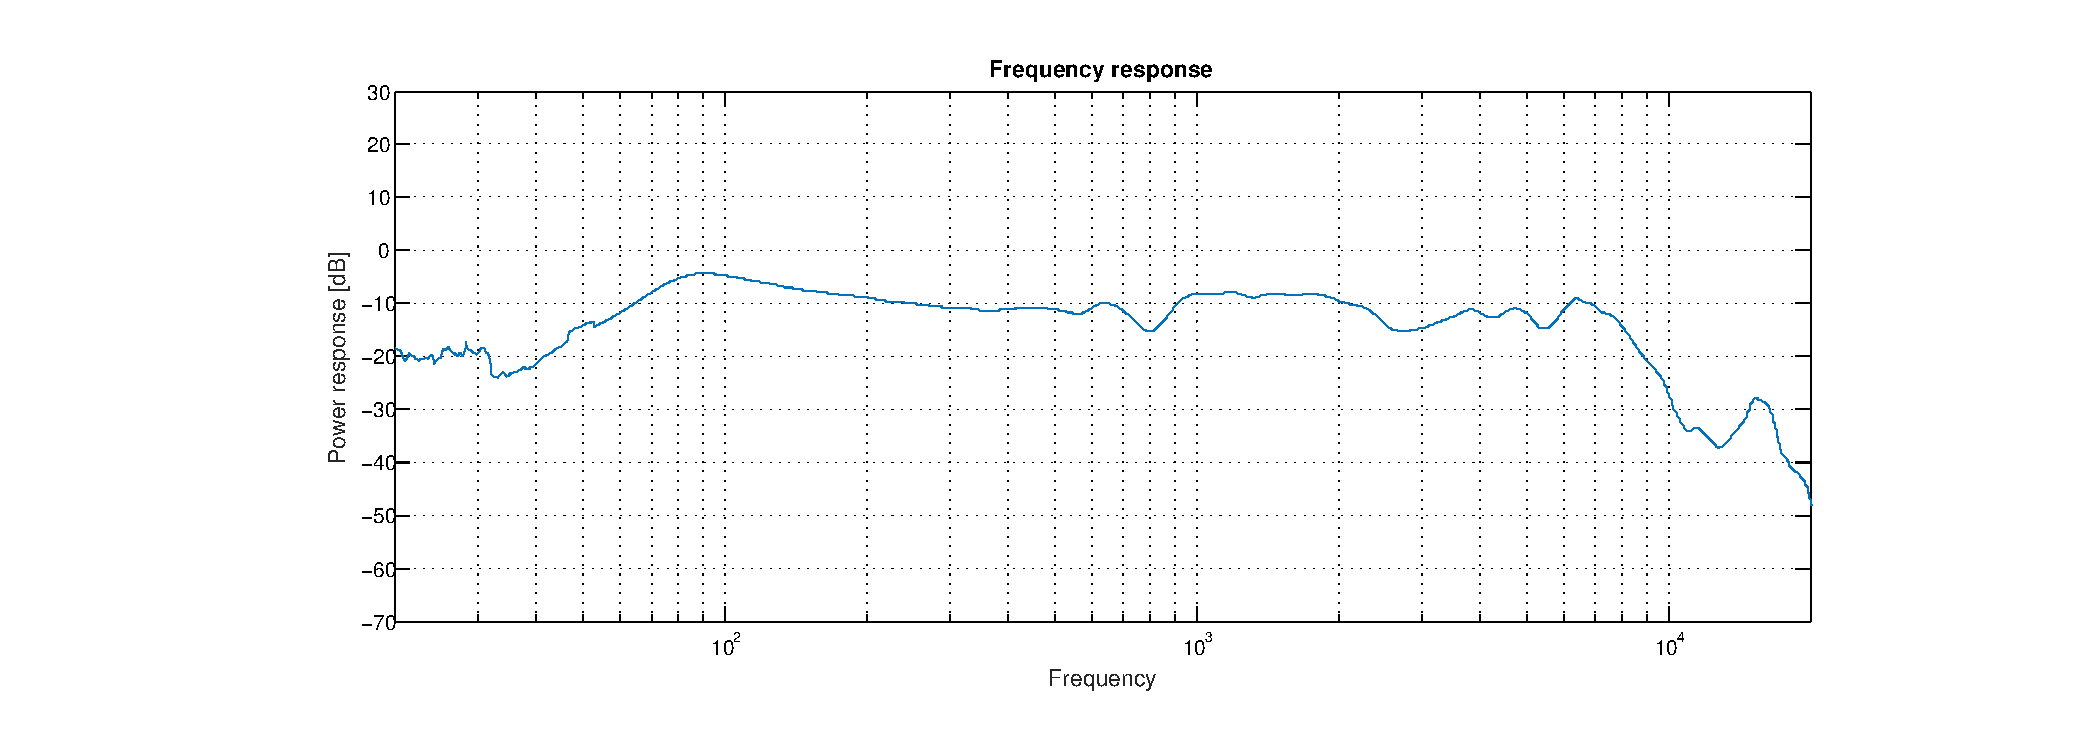
\includegraphics[height=0.2\paperheight]{Figures/Mid_Response_JBT}%
  }
\caption{Frequency response of the the speakers}
\label{fig:Calculated_impedance_models_fitted}
\end{figure}

\subsubsection{Results}
The results obtained were what was approximately expected from the tests, these can be observed in appendix C4 and C5. Both the frequency response and the phase shift for all the different components will be mentioned there. For the tweeter, the higher frequencies really came alive and the phase shift was very clear in the higher frequencies. The mid-range was rather confusing, as can bee seen from the figure 4 on the previous page. It has an overall good sound signature and the phase shift was readable throughout most frequencies ranges, except for the very high frequencies. The woofers on the other hand were a bit confusing. Their phase shift was very clear however, the frequency response they gave was rather confounding. They performed bad on the low frequencies and even worse on the higher frequencies. Nevertheless, this could be due to the bad quality of the microphone, speaking of which, always gave the same frequency response from 1Hz up to 15Hz. The only difference with the speakers was the magnitude of the sound at this range.

\begin{figure}
 \centering
  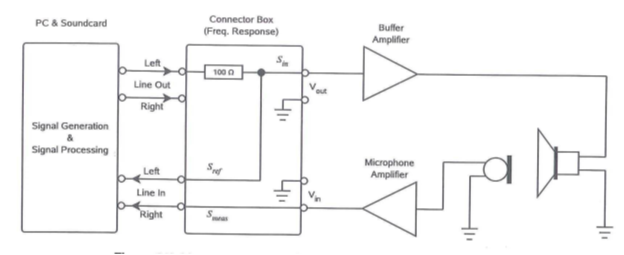
\includegraphics[width=0.9\textwidth]{Figures/Setup}
  \caption{Measurement setup for short distance }
  \label{fig:shortdistancemeasurement}
\end{figure}


\newpage
\subsection{Impedance Measurement}
\subsubsection{Setting-up}
To measure the impedance of a speaker, as mentioned earlier, we used the LS\textsubscript{Measure} program. The white noise is used as input of a voltage divider (connection box) consisting of a high accuracy resistor of 100 Ohm. A jack-jack cable connects the line-out of the PC to the line-out connector of the connection box. The same method is used to connect the line-in. 
\newline
As reference, we chose the integrated resistor in the connection box which is 100 OHM. Also, the V\textsubscript{out} and V\textsubscript{in} of the connection box were connected to the input and output of the respective speakers. Since the low speaker consists of two separated components, therefore they must be connected in parallel and eventually connected back to the connection box. The topology of the circuit is shown in figure 4 [1].       

\begin{figure}[H]
  \centering
  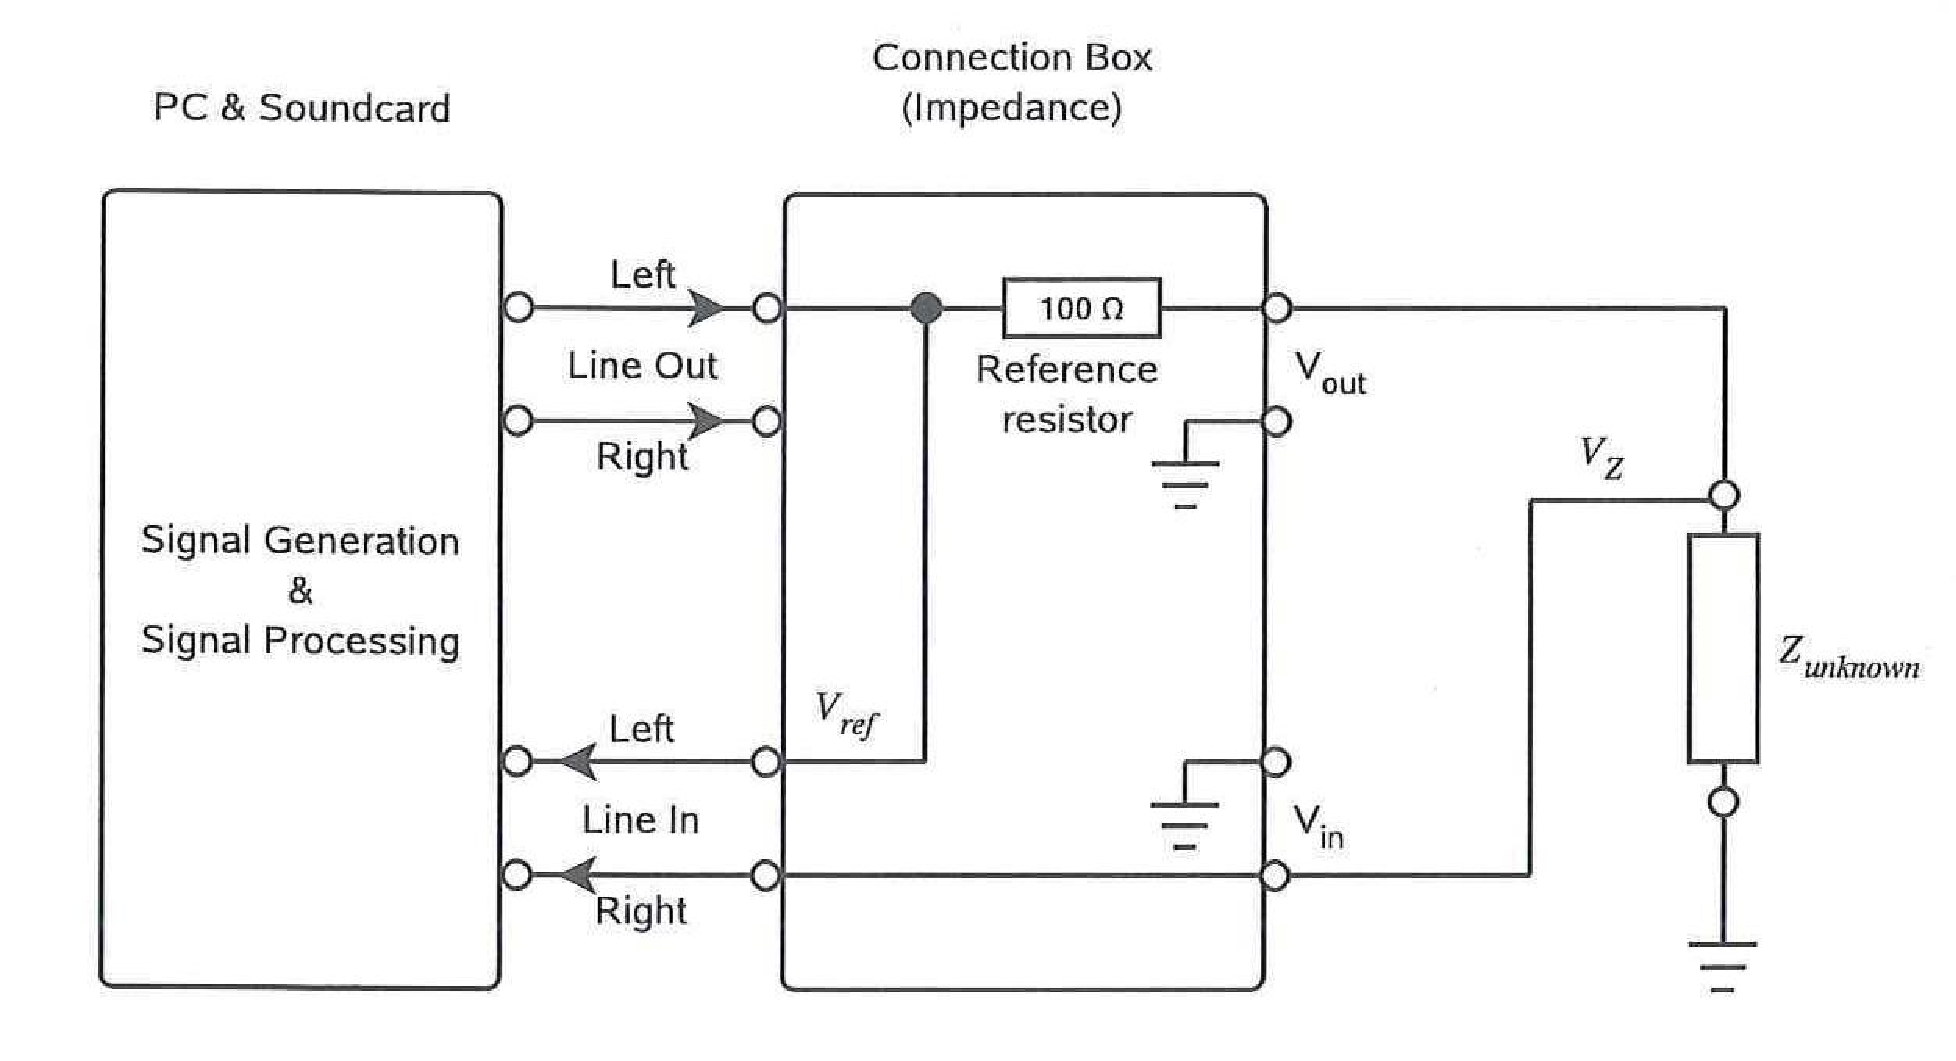
\includegraphics[width=0.8\textwidth]{Figures/setup_elec_cropped.pdf}
  \caption{Measurement setup for measuring impedances}
  \label{fig:setupelec}
\end{figure}

\subsubsection{Measurement Procedure}
Assuming the setup has been set correctly. A white noise is generated from the PC and is used as input of a voltage divider. Both the generated noise signal ($V_ref$) and the voltage V\textsubscript{Z} over the unknown impedance Z\textsubscript{unknown} are eventually fed back into the PC. With this data, the program LS\_measure can then determine the value of Z\textsubscript{unknown}. This is done with equation 1. With the LS\_measure program we could then obtain the frequency response graph. Initially the program must be set in the correct configuration. All this meant, was that the sample frequency had to be set at 48 kHz and the ML-generator length at 18. 

\begin{equation}
 Z_{Unknown}(f)= \frac{R_{ref} \cdot V_{Z}(f)}{V_{ref}(f) - V_{z}(f)} 
\end{equation}
\indent
Equation 1 [1] is used by $LS_{measure}$ to calculate the unknown impedances.

\section{Conclusion}
The purpose to conduct the calculations and measurements for the impedance is to find electrical impedance models of the speaker. These can then be used to create zobel networks for the filters according to these values. The frequency response is needed to locate the proper cut-off frequency for each component. This data can thus also be used to design the filters. 
\begin{table}[ht] % another one DEEE JAYYY KHALEEEEEEEEEEEED
  \centering
  \begin{tabular}{p{1.3cm} >{\centering\arraybackslash}p{1.3cm} >{\centering\arraybackslash}p{1.3cm} >{\centering\arraybackslash}p{1.3cm}}
    \toprule
     & \textbf{low} & \textbf{mid} & \textbf{high} \\
    \midrule
    $R_e\ (\si{\ohm})$          & 4.00 & 3.70  & 4.30 \\ 
    $L_e\ (\si{\micro\henry})$  & 922  & 437   & 74.2 \\
    $R_p\ (\si{\ohm})$          & 12.6 & 6.88  & 4.31 \\
    $C_p\ (\si{\micro\farad})$  & 808  & 1513  & 71.6 \\ 
    $L_p\ (\si{\micro\henry})$  & 6844 & 2456  & 519  \\
    \bottomrule
  \end{tabular}
  \caption{Component values repeated}
  \label{tab:componentvaluesrepeated}
\end{table}

The values in the table above show all the different values for the components of the speaker impedance model. The woofer and mid-range both have very high values for $L_e$, $C_p$, and $L_p$. This is due to the required frequency range at which these components have to play. This range includes the resonant frequency, which is very hard to cope with and therefor have very high values for these electrical segments. However, this is a simplified model, the real model is much more complicated. Nevertheless, it is representative enough for us to cope with and further calculate with. 

\section{Recommendations}
Let us now take a step back and re-evaluate the strategies we could use to improve the obtained results. As for the acoustic response measurement we did not possess a microphone of high quality, this affected the measured results in a negative way.
\newline
The impedance improvement could have been improved by increasing the ML-generator length. Nonetheless, this was not possible with the computing power of the desktops at the university. It simply would have taken too long to do these measurements. Furthermore, it would have been worth the time waiting for the increase in quality. 

\section{Bibliography}
\bibliographystyle{plain}
\bibliography{books}

\newpage\appendix
\part*{Appendices}\label{part:appendices}
\addcontentsline{toc}{section}{Appendices}
\renewcommand{\thesection}{\Alph{section}}

\section{Derivations}\label{app:deriv}
The first value that can be retrieved from the measured impedance's at different frequencies is the value of $R_p$. At the resonance peak, the impedance of the speaker is equal to $R_e + R_p$, assuming that the impedance of the self-inductance is negligible there, thus:
\begin{align*}
    Z_{ls}(\omega_0) &= R_e + R_p\\
    R_p              &= Z_{ls}(\omega_0) - R_e
\end{align*}
At resonance, $Z_{ls} = \abs{Z_{ls}}$, thus:
\begin{equation}
 R_p = \abs{Z_{ls}(\omega_0)} - R_e\label{eq:rp}
\end{equation}

To calculate $C_p$, the formula for the bandwidth of a resonance circuit is used. The bandwidth can be determined from the graph as it is defined as the distance between both sides of the resonance peak where the impedance is given by $\frac{R_p}{\sqrt{2}}$. The bandwidth can also be calculated from the resonance circuit values. Thus:
\begin{align}
  B_w                 &= \frac{1}{C_p \cdot R_p}\nonumber\\
  B_w (C_p \cdot R_p) &= 1\nonumber\\
  C_p \cdot R_p       &= \frac{1}{B_w}\nonumber\\
  C_p                 &= \frac{1}{B_w \cdot R_p}\label{eq:cp}
\end{align}

With the calculated value of $C_p$ and with the measured value of the resonance frequency, the value of $L_p$ can be computed, by rewriting the formula for the resonant frequency:
\begin{align*}
  \omega_0                   &= \sqrt{\frac{1}{C_p \cdot L_p}}\nonumber\\
  \omega_0^2                 &= \frac{1}{C_p \cdot L_p}\nonumber\\
  \omega_0^2 (C_p \cdot L_p) &= 1\nonumber\\
  C_p \cdot L_p              &= \frac{1}{\omega_0^2}\nonumber\\
  L_p                        &= \frac{1}{\omega_0^2 \cdot C_p}
\end{align*}

Note that the resonance frequency is an angular frequency (this can be calculated by $\omega = 2\pi f$). The rewritten equation is as follows:
\begin{equation}
  L_p = \frac{1}{\omega_0^2 \cdot C_p}\label{eq:lp}
\end{equation}

To calculate the value of $L_e$, one can make use of the observation that at frequencies well above the resonant frequency, the impedance approaches the impedance of $R_e$ and $L_e$. Rewriting yields:
\begin{align}
  Z_{ls}         &= R_e + j \omega L_e\nonumber\\
  \abs{Z_{ls}}   &= \abs{R_e + j \omega L_e}\nonumber\\
  \abs{Z_{ls}}   &= \sqrt{R_e^2 + (\omega L_e)^2}\nonumber\\
  \abs{Z_{ls}}   &= \sqrt{R_e^2 + \omega^2 L_e^2}\nonumber\\
  \abs{Z_{ls}}^2 &= R_e^2 + \omega^2 L_e^2\nonumber\\
  L_e^2          &= \frac{\abs{Z_{ls}}^2 - R_e^2}{\omega^2}\nonumber\\
  L_e            &= \sqrt{\frac{\abs{Z_{ls}}^2 - R_e^2}{\omega^2}}\label{eq:le}
\end{align}

Here, $\abs{Z_{ls}}$, and $\omega$ are values obtained from a point from the impedance measurements. Since this formula holds mainly for frequencies much higher then the resonance peak, the point should be chosen at such a frequency.

\newpage\section{Course-lab exercises}
Answers to the exercises found in the student course labs manual. \cite{studentmanual}
\subsection{Exrcises on page 131}
As we saw from figures of the MatLab code from tutorial 2, at low frequencies
a capacitor behaves as a low-pass filter. In other words, it passes the low frequencies through and rejects the high frequencies. The phase difference in these circuits is minimal for the lower frequencies and increases to a maximum of 90 degrees for higher frequencies. The phase difference and frequency response both decrease or increase respectively at the same cut-off point.
\newline
If the resistance in an RC circuit is lowered, the cutoff frequency will be higher.
\newline
In contrast, the inductor does not let low frequencies through ,because it works as a high-pass filter.
\newline
What we also saw from the figures of the MatLab code is that at high frequencies, 
an inductor behaves as a high-pass filter, which is the opposite of how a capacitor works. The phase difference is therefore also opposite to that of the capacitor, having minimal phase difference at the higher frequencies and increasing towards the lower frequencies.
\newline
Lowering the resistance in an RL circuit will lower the cut-off frequency.
\newline
\subsection{extra questions on page 112} 
the maximum frequency of the measuring system is determined by the sampling frequency. This frequency in LS-measure was set to 48kHz, therefor the maximum frequency which could be measured was 24kHz.
\newline
Resonance is a condition in an RLC circuit in which the inductive and capacitive reactants are equal in magnitude,thereby resulting in a purely resistive impedance. It is the cause of oscillations of stored energy from one form to another. 

\newpage\section{Matlab scripts}
\subsection{Circuit simulation}
This page contains  the MatLab script used to model the circuit. Note that the script makes use of external *.mat and *.fig files To load specific data, the file names in the 'load()' and 'openfig()' functions should be changed.
\begin{lstlisting}
% Speaker model procedure (EPO-1 assignment)
%
% A speaker can be modeled with a resistance Re, an inductance Le, 
% and an electrical model for a mass spring system in series. The 
% mass spring system is modeled with a capacitor Cp, an Inductance 
% Lp and a resistor Rp in series. 
% This script models the circuit's impedance. 
% For the values of Re, Le, Cp, Lp and Rp values calculated from 
% measurements made during EPO are used.
% 
% Author: Rietveld, Jasper, 16 November 2016

% Firstly, the values of Re, Le, Rp, Cp and Lp are loaded into the 
% program from a matlab file. The values are optionally overwritten 
% by values obtained from the function fit by uncommenting line 18.

load('values full model bass calculated');
% load('values full model bass fit');

% The program also opens the figure containing the measurements.
% This way, the model values can be plotted together with the 
% measurements for comparison.
openfig('Impedance Amplitude BASS.fig');
hold on;

% A logspace for the frequencies is created.
f = logspace(1,log(20000),48000);

% The impedance is calculated with the formula as obtained in
% section 2 of the report
Z = abs(Re + 1j*2*pi*f*Le + 1./(1/Rp + 1j*(2*pi*f)*Cp + 1./(1j*2*pi*f*Lp)));

% The results are then drawn to a plot with the right lables 
% attached to it.
semilogx(f, Z)
ylim([0 20])
grid on
title('Impedance Amplitude')
xlabel('frequency [Hz]')
ylabel('Impedance [|Z|]')
legend('Measured values','Model values','Location','SouthEast')

% Optionally the graph can be saved as an eps file to use in 
% LaTeX documents by uncommenting line 46

% print -depsc Bass_model_calculated
\end{lstlisting}

\newpage\subsection{Function fit}
This page contains  the MatLab script used to conduct the function fit. Note that the script makes use of external *.mat and *.fig files To load specific data, the file names in the 'load()' and 'openfig()' functions should be changed.
\begin{lstlisting}
% function fit (EPO-1 assignment)
%
% This script executes a function fit based on a custom fittype 
% and input data obtained from a graph. The fittype has been made
% specifically to calculate values for the impedance model.
% The resulting variables are also immediatly plotted for ease of use.
% 
% Author: Rietveld, Jasper, 24 November 2016

% To start, the Data to fit the function to is loaded by opening
% the corresponding figure
openfig('Impedance Amplitude HIGH.fig');
hold on;

% To improve the program's performance, certain start and end 
% limits may be chosen
Start = 10^2.4;
End = 20000;

% To improve the program's performance, values for the parameters
% (in this case component values) can be used as starting points.
% this can be done by uncommenting line 24-35

% load('values full model high calculated');

% Le_s = Le;
% Cp_s = Cp;
% Lp_s = Lp;
% Rp_s = Rp;
% Re_s = Re;
% clear Rp;
% clear Re;
% clear Le;
% clear Cp;
% clear Lp;

% Next, a fittype is created for the impedance model.
% Some values may not need to be fitted. These values should be 
% filled into the fittype and be removed from the 'coefficients'
% array. The bounds and limits on line x should also be removed.

ft = fittype('abs(Re+1j*2*pi*f*Le+1/(1/Rp+1j*(2*pi*f)*Cp+1./(1j*2*pi*f*Lp)))',...
   'independent',{'f'y},...
   'coefficients',{'Le','Cp','Lp','Re','Rp'}...
   );

% In order to be able to fit the function to the data in the
% matlab figure, the X and Y vectors need to be extracted from
% the figure. This is done next.

D=get(gca,'Children'); %get the handle of the line object.
XData=get(D,'XData'); %get the x data.
YData=get(D,'YData'); %get the y data.

% the X and Y vectors of the input data are then shortened to
% the start and end values.
selector = (XData > Start) & (XData < End);
XData = XData(selector);
YData = YData(selector);

% Then, the new shortened X and Y data is plotted again.
close all;
semilogx(XData,YData)
xlim([Start End])
hold on;

% Next the function fit is executed.
f=fit(XData(:),YData(:),ft,...
  'StartPoint',[Le_s, Cp_s, Lp_s, Re_s, Rp_s],...
  'Lower',[0,0,0,0,0]);

% After the function fit is done, the results are plotted.
grid on;
plot(f)
\end{lstlisting}

\newpage\subsection{Relative deviation calculations}
This page contains  the MatLab script used to conduct relative deviation calculations. Note that the script makes use of external *.mat and *.fig files To load specific data, the file names in the 'load()' and 'openfig()' functions should be changed.
\begin{lstlisting}
% Relative deviation calculations (EPO-1 assignment)
%
% This script calculates and plots the relative deviation of the
% impedance model with certain values on a certain domain as a
% percentage of the measured data and plots it as a graph. Apart
% from that, the script also calculated the average relative
% deviation over the domain.
% 
% Author: Rietveld, Jasper, 2 december 2016

% Firstly, the values of Re, Le, Rp, Cp and Lp are loaded into the 
% program from a matlab file.
load('values full model mid calculated');
openfig('Impedance Amplitude MID.fig');
hold on;

% determine the start and end points of the domain to be evaluated.
Start = 300;
End = 1900;

% In order to be able to fit the function to the data in the
% matlab figure, the X and Y vectors need to be extracted from
% the figure. This is done next.

D=get(gca,'Children'); %get the handle of the line object.
XData=get(D,'XData'); %get the x data.
YData=get(D,'YData'); %get the y data.

% the X and Y vectors of the input data are then shortened to
% the start and end values.
selector = (XData > Start) & (XData < End);
XData = XData(selector);
YData = YData(selector);

% The impedance is then calculated with the formula as obtained in
% section 2 of the report
Z_Calculated = abs(Re + 1j*2*pi*XData*Le + 1./(1/Rp + 1j*(2*pi*XData)*Cp + 1./(1j*2*pi*XData*Lp)));
Zero = zeros(1,length(YData));

% After that, the relative deviation is calculated based on the
% measured impedance and the calculated modeled impedance.
Relative_Deviation_Calculated = Z_Calculated./YData*100 - 100;

% The average deviation is calculated by taking the integral 
% of the function and calculating it's average.
Average_Deviation_Calculated = (trapz(XData,abs(Relative_Deviation_Calculated)))/(End-Start);

% The values of the calculation are then overwritten by values obtained from 
% the function fit, and the calculations are repeated.

load('values full model mid fit');

Z_Fitted = abs(Re + 1j*2*pi*XData*Le + 1./(1/Rp + 1j*(2*pi*XData)*Cp + 1./(1j*2*pi*XData*Lp)));
Zero = zeros(1,length(YData));

Relative_Deviation_Fitted = Z_Fitted./YData*100 - 100;

Average_Deviation_Fitted = (trapz(XData,abs(Relative_Deviation_Fitted)))/(End-Start);

% The results are then plotted in two subplots, one containing
% the impedance measurements and the other one containing
% the relative deviation.
close all;

subplot(211)
semilogx(XData, YData)
hold on;
semilogx(XData, Z_Calculated)
semilogx(XData, Z_Fitted)
legend('Measured values','Model values','Fitted values','Location','NorthEast')
grid on;
xlabel('frequency [Hz]')
ylabel('Impedance [|Z|]')
ylim([0 20])
xlim([Start End])

subplot(212)
semilogx(XData, Zero)
hold on;
semilogx(XData, Relative_Deviation_Calculated)
semilogx(XData, Relative_Deviation_Fitted)
legend('no deviation','Model deviation','Fitted values','Location','NorthEast')
grid on;
xlabel('frequency [Hz]')
ylabel('Relative deviation [%]')
ylim([-100 100])
xlim([Start End])

% The resulting values of the average deviation are also printed to the
% command window.
Average_Deviation_Calculated
Average_Deviation_Fitted
\end{lstlisting}

\newpage\section{Matlab figures}
\subsection{model from calculations}
\begin{figure}[H]
\centering
\subcaptionbox{Bass model from calculations\label{fig:Bass_Impedance_Model_Calculated}}{%
  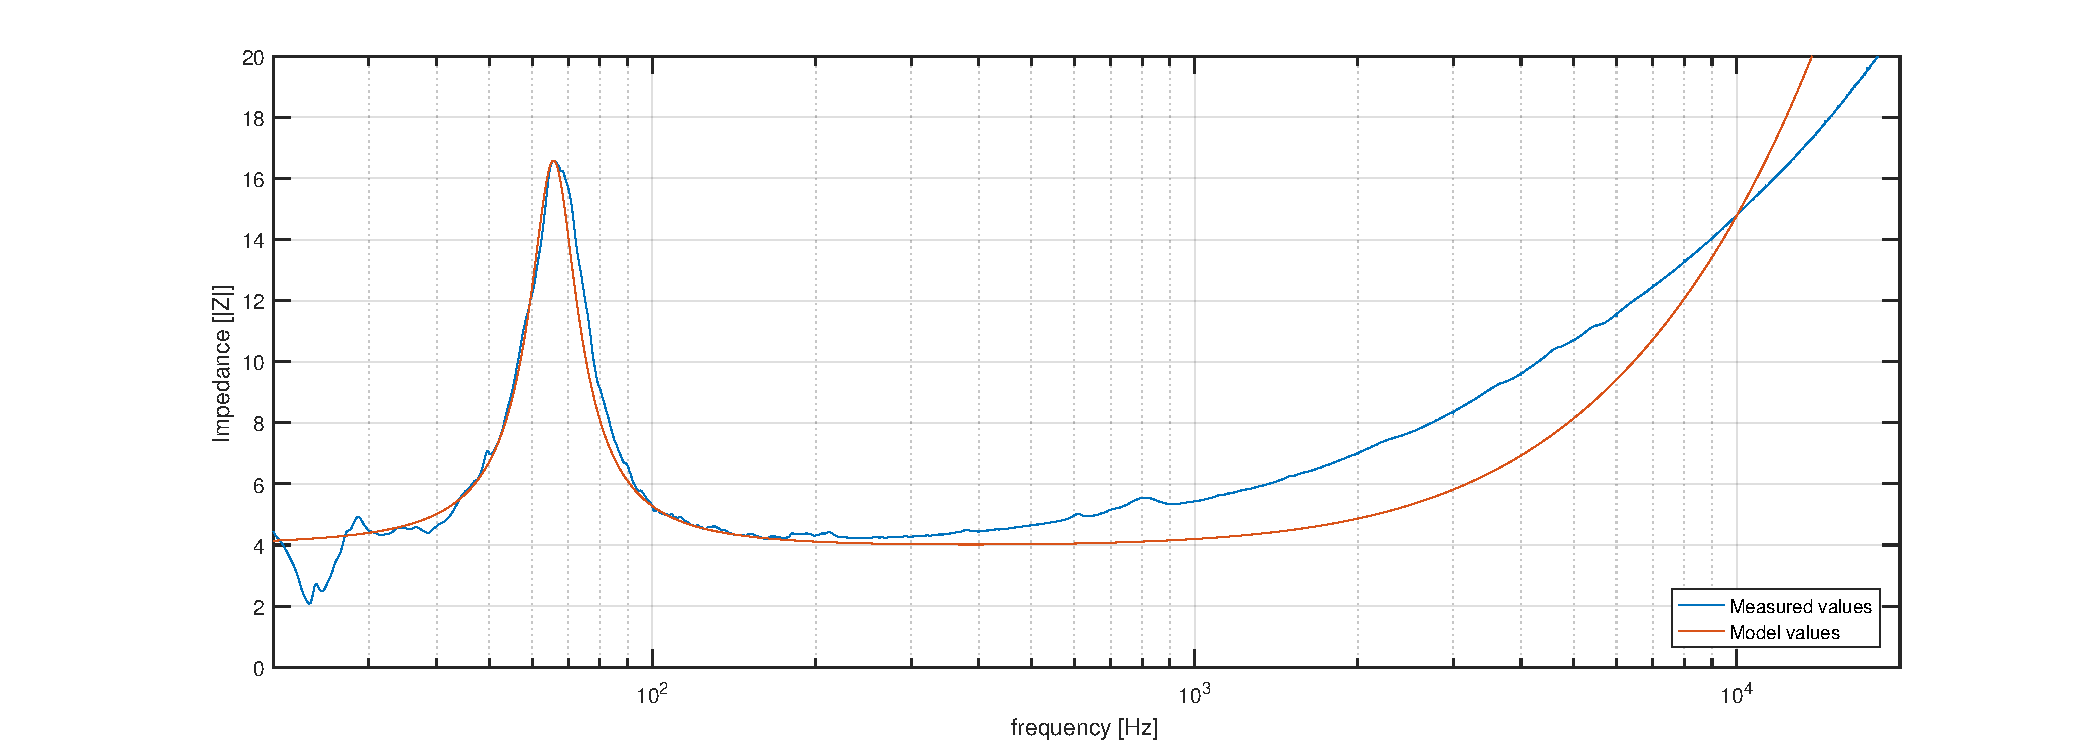
\includegraphics[height=0.2\paperheight]{Figures/Bass_Impedance_Model_Calculated}%
  }\par\medskip
\subcaptionbox{Mid model from calculations\label{fig:Mid_Impedance_Model_Calculated}}{%
  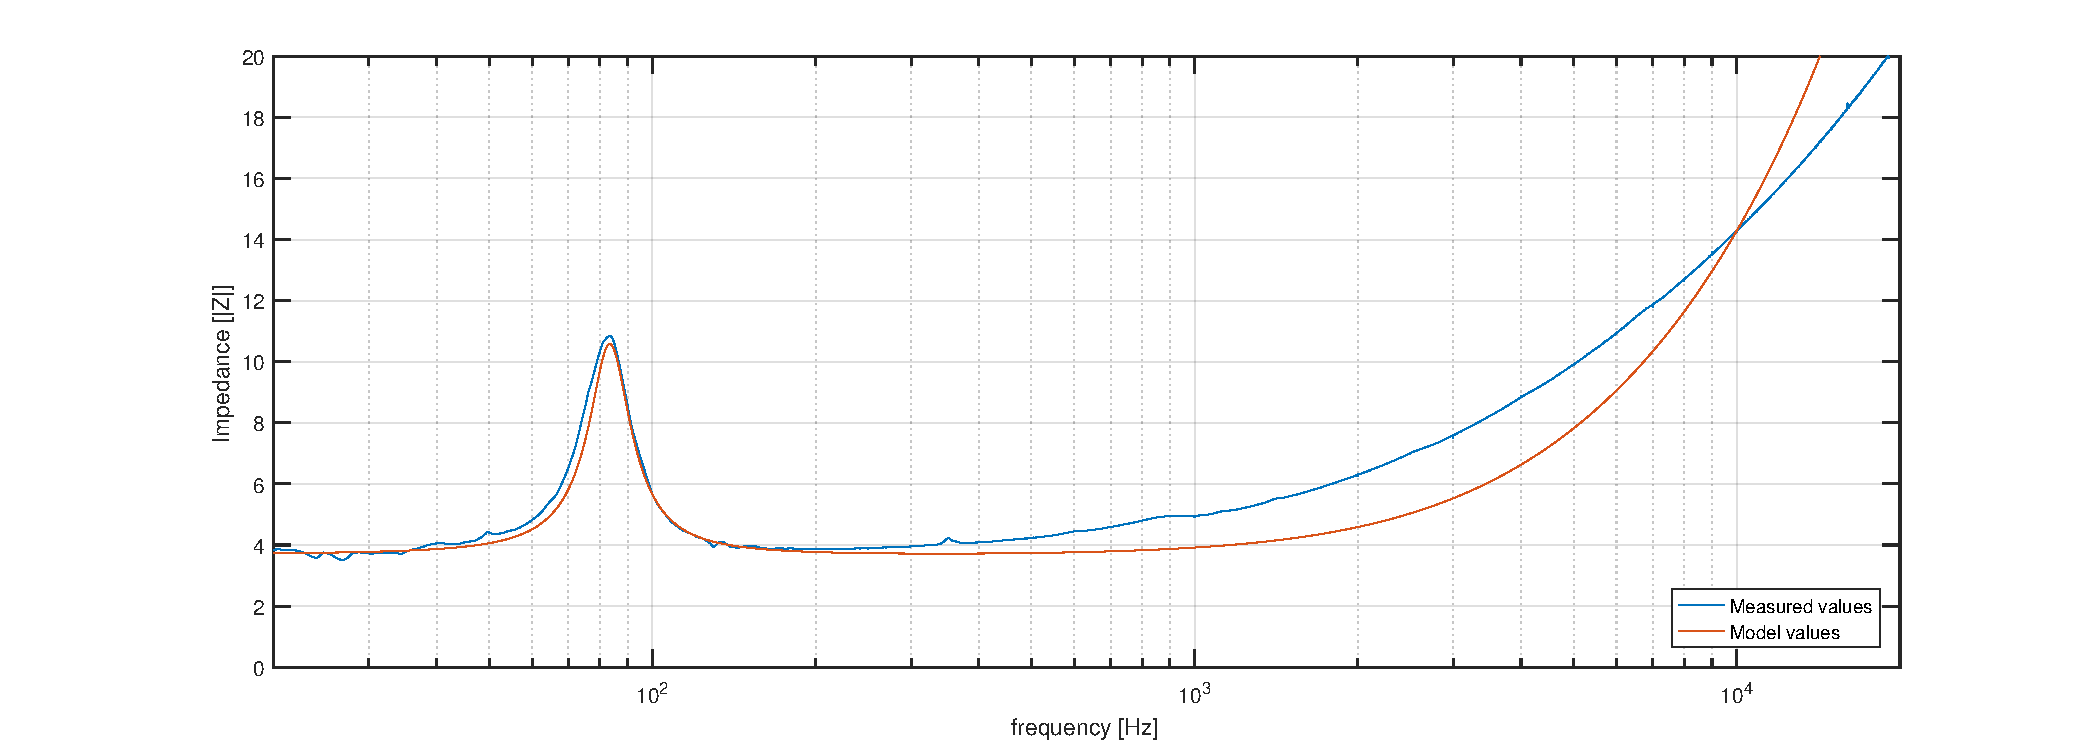
\includegraphics[height=0.2\paperheight]{Figures/Mid_Impedance_Model_Calculated}%
  }\par\medskip        
\subcaptionbox{High model from calculations\label{fig:High_Impedance_Model_Calculated}}{%
  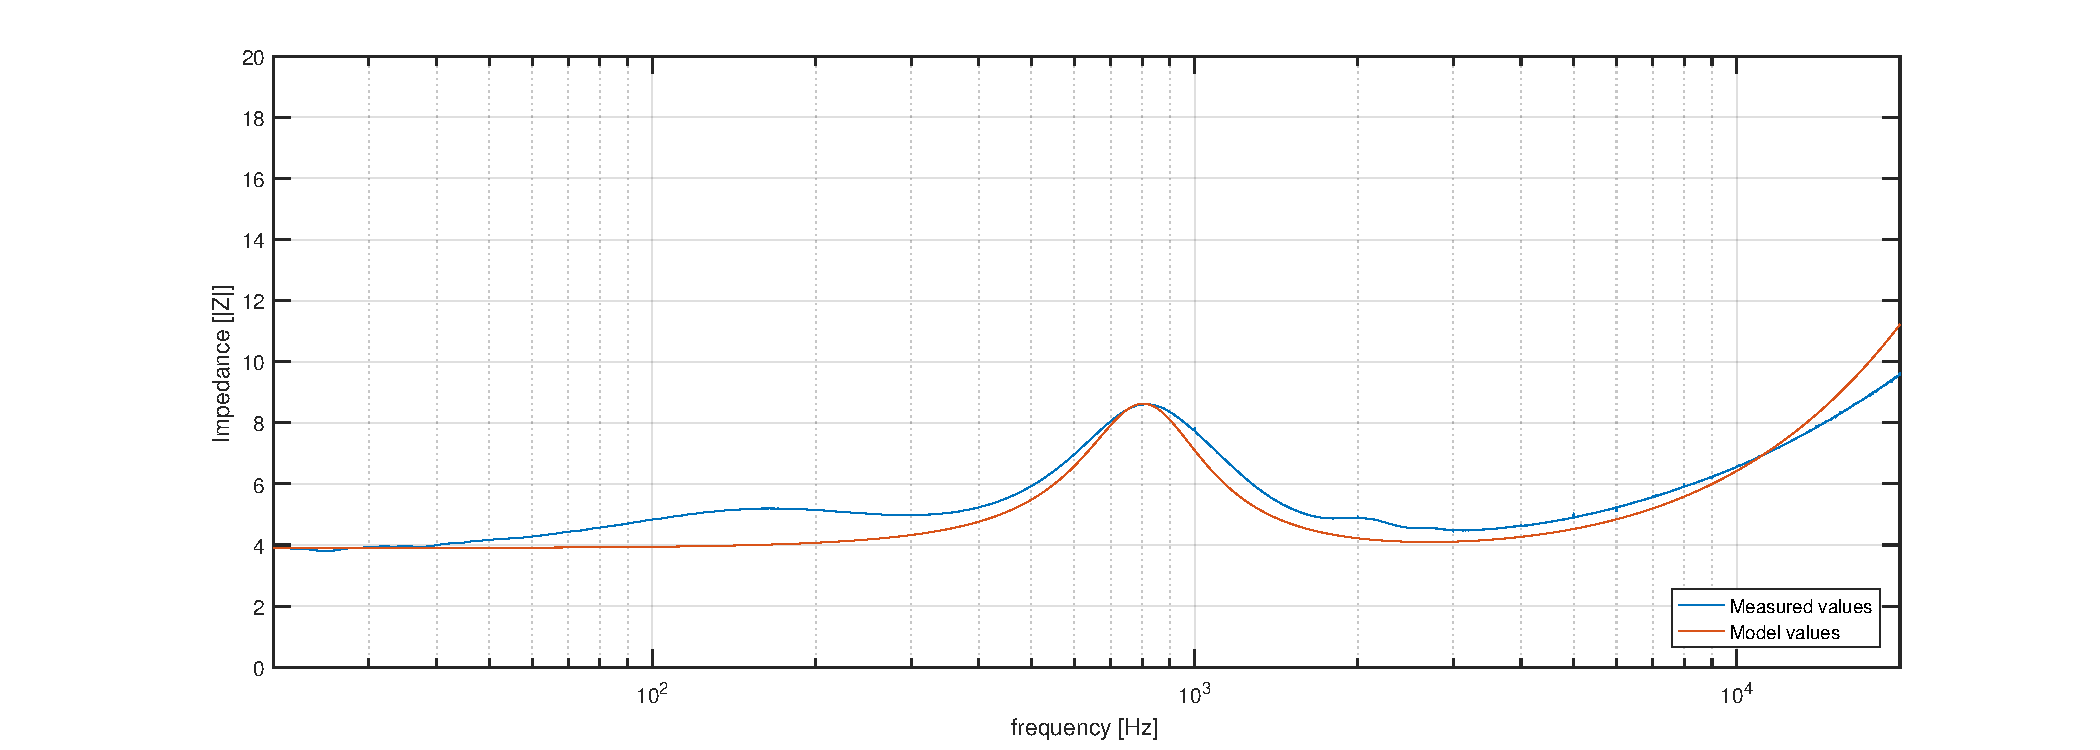
\includegraphics[height=0.2\paperheight]{Figures/High_Impedance_Model_Calculated}%
  }
\caption{Impedance models based on calculated component values}
\label{fig:Calculated_impedance_models_calculated}
\end{figure}

\newpage
\subsection{model from function fit values}
\begin{figure}[H]
\centering
\subcaptionbox{Bass model from function fit\label{fig:Bass_Impedance_Model_Fitted}}{%
  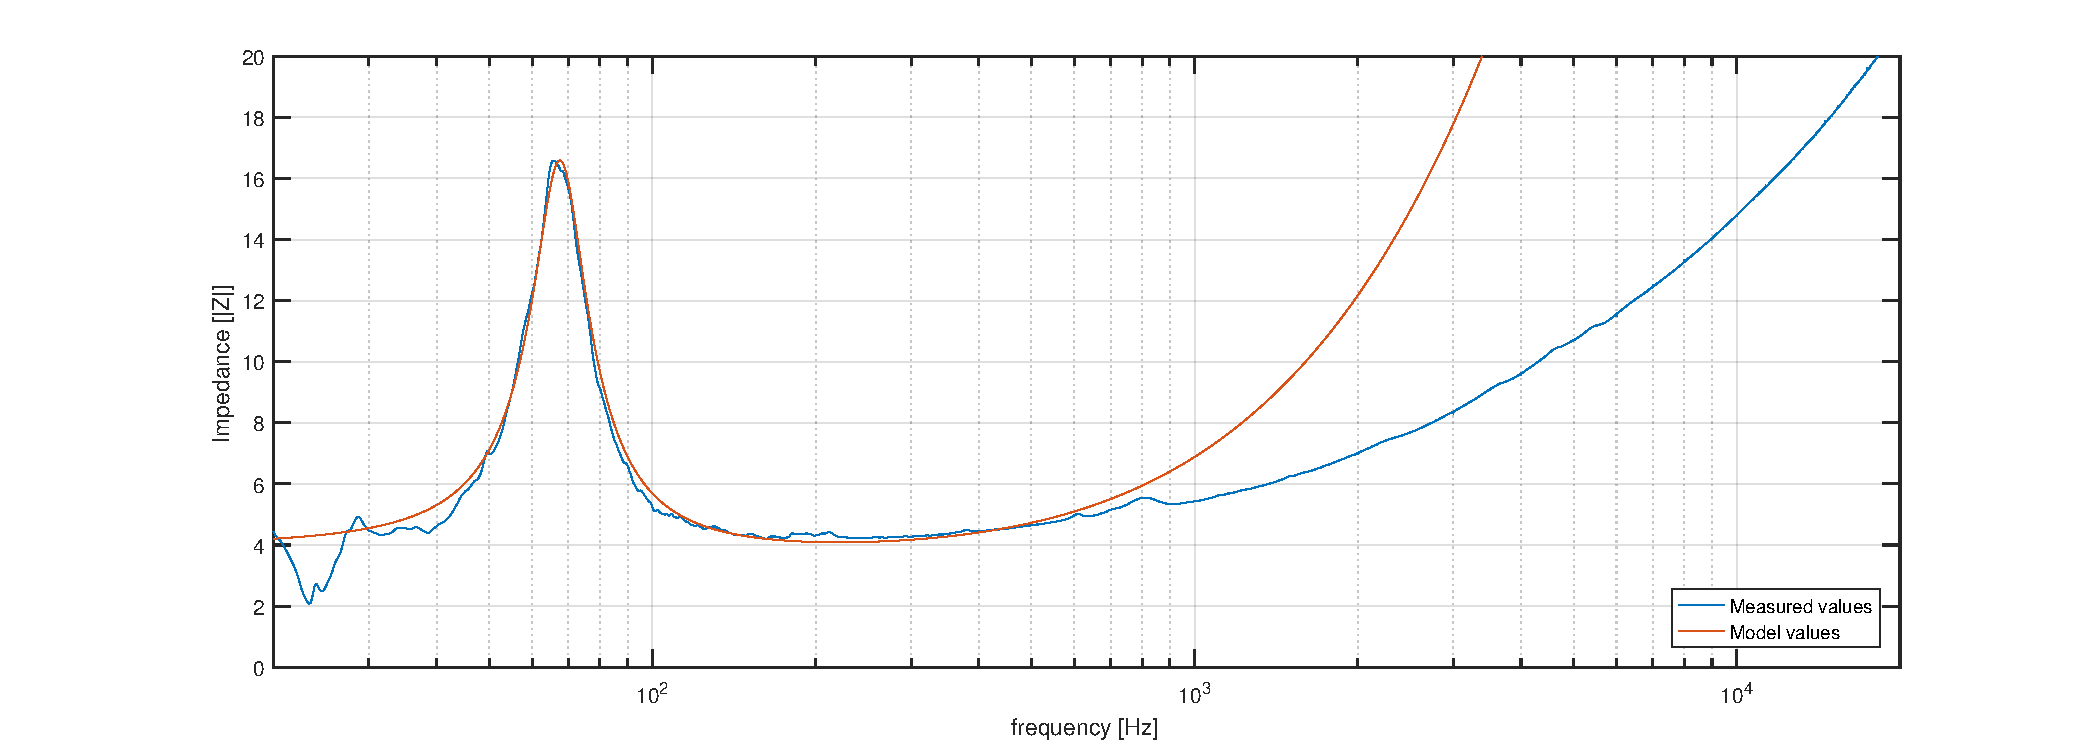
\includegraphics[height=0.2\paperheight]{Figures/Bass_Impedance_Model_Fitted}%
  }\par\medskip
\subcaptionbox{Mid model from function fit\label{fig:Mid_Impedance_Model_Fitted}}{%
  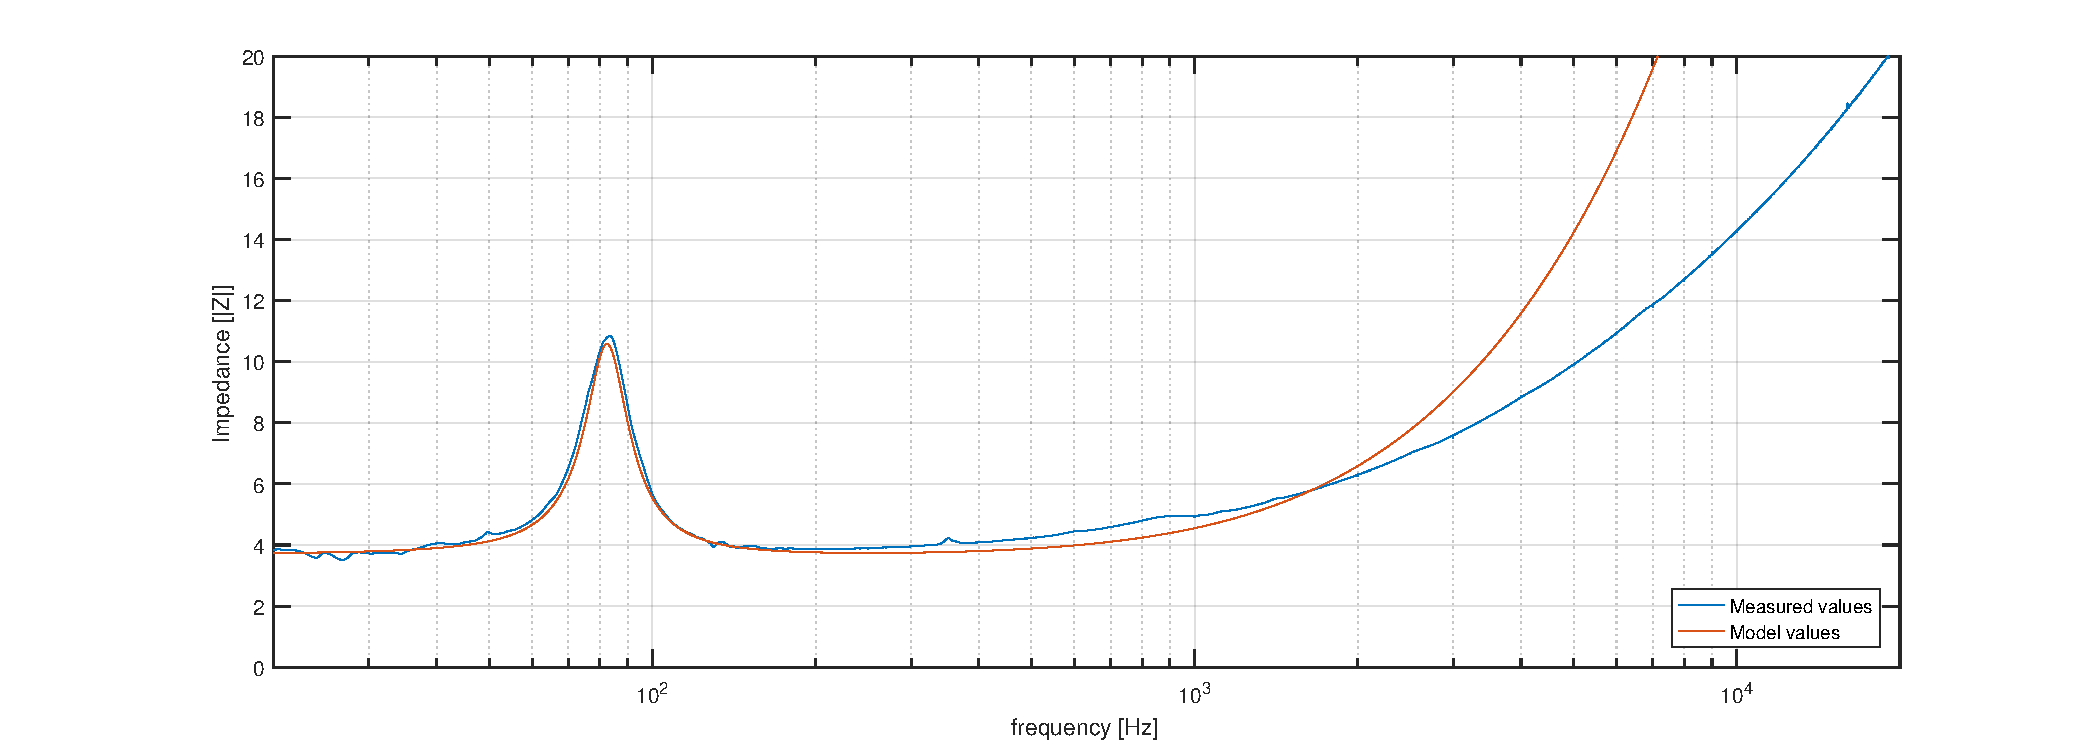
\includegraphics[height=0.2\paperheight]{Figures/Mid_Impedance_Model_Fitted}%
  }\par\medskip        
\subcaptionbox{High model from function fit\label{fig:High_Impedance_Model_Fitted}}{%
  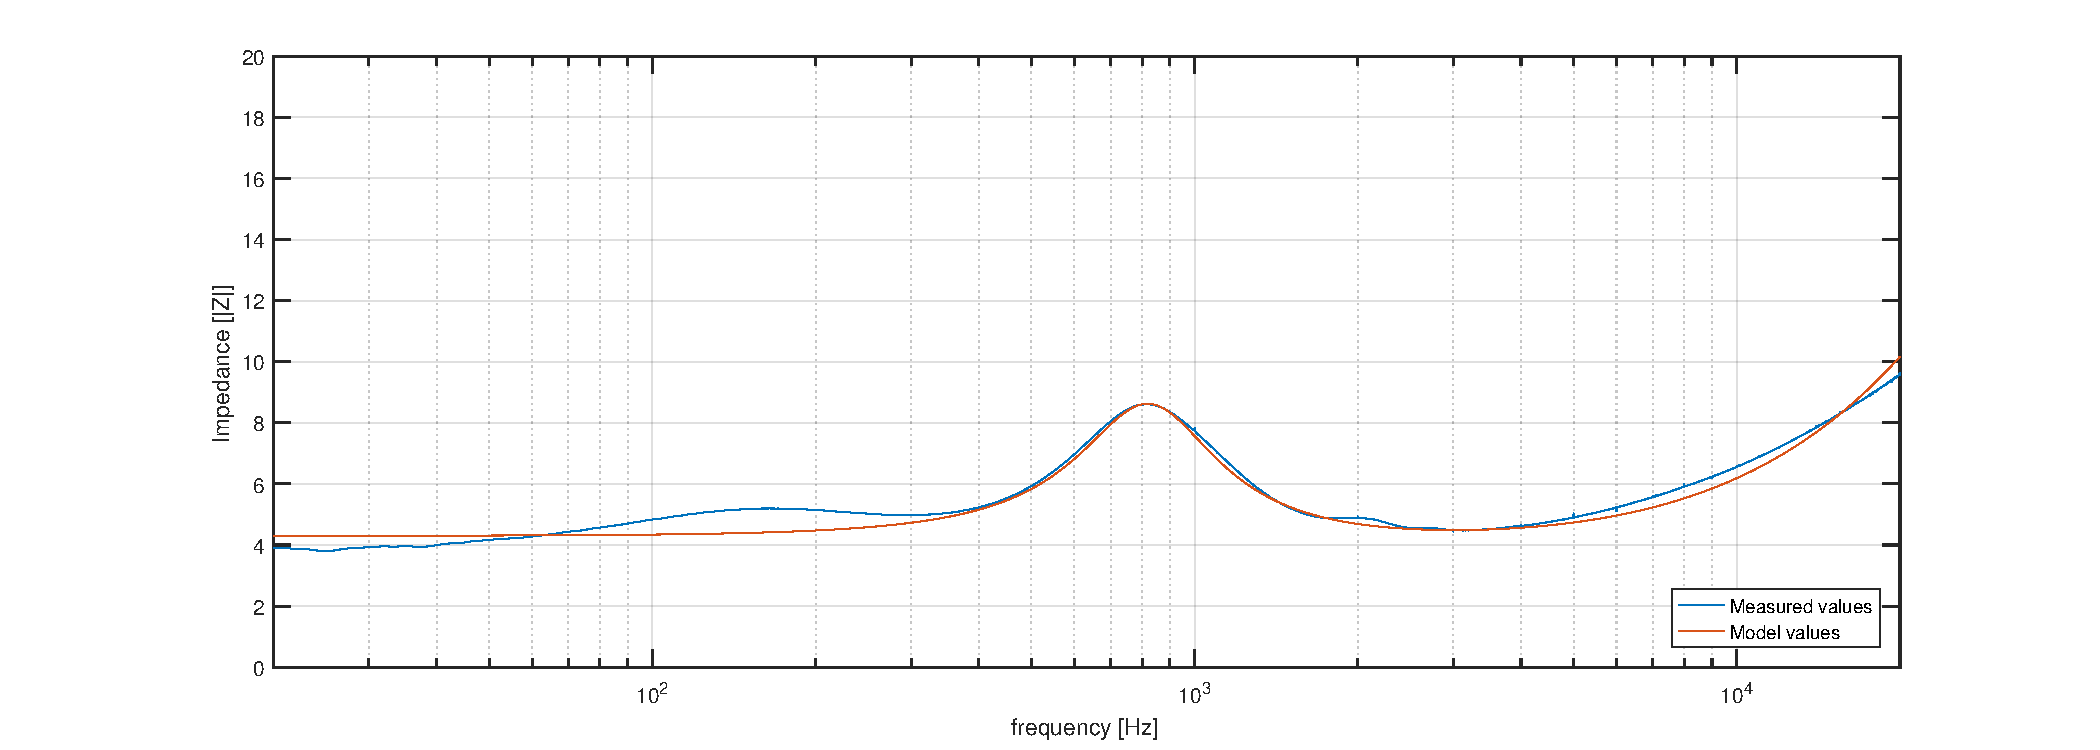
\includegraphics[height=0.2\paperheight]{Figures/High_Impedance_Model_Fitted}%
  }
\caption{Impedance models based on calculated component values}
\label{fig:Calculated_impedance_models_fitted}
\end{figure}

\newpage
\subsection{relative deviation calculation graphs}
\begin{figure}[H]
\centering
\subcaptionbox{Relative deviations of the models for the bass speakers\label{fig:Relative_Deviation_Bass_Impedance_Models}}{%
  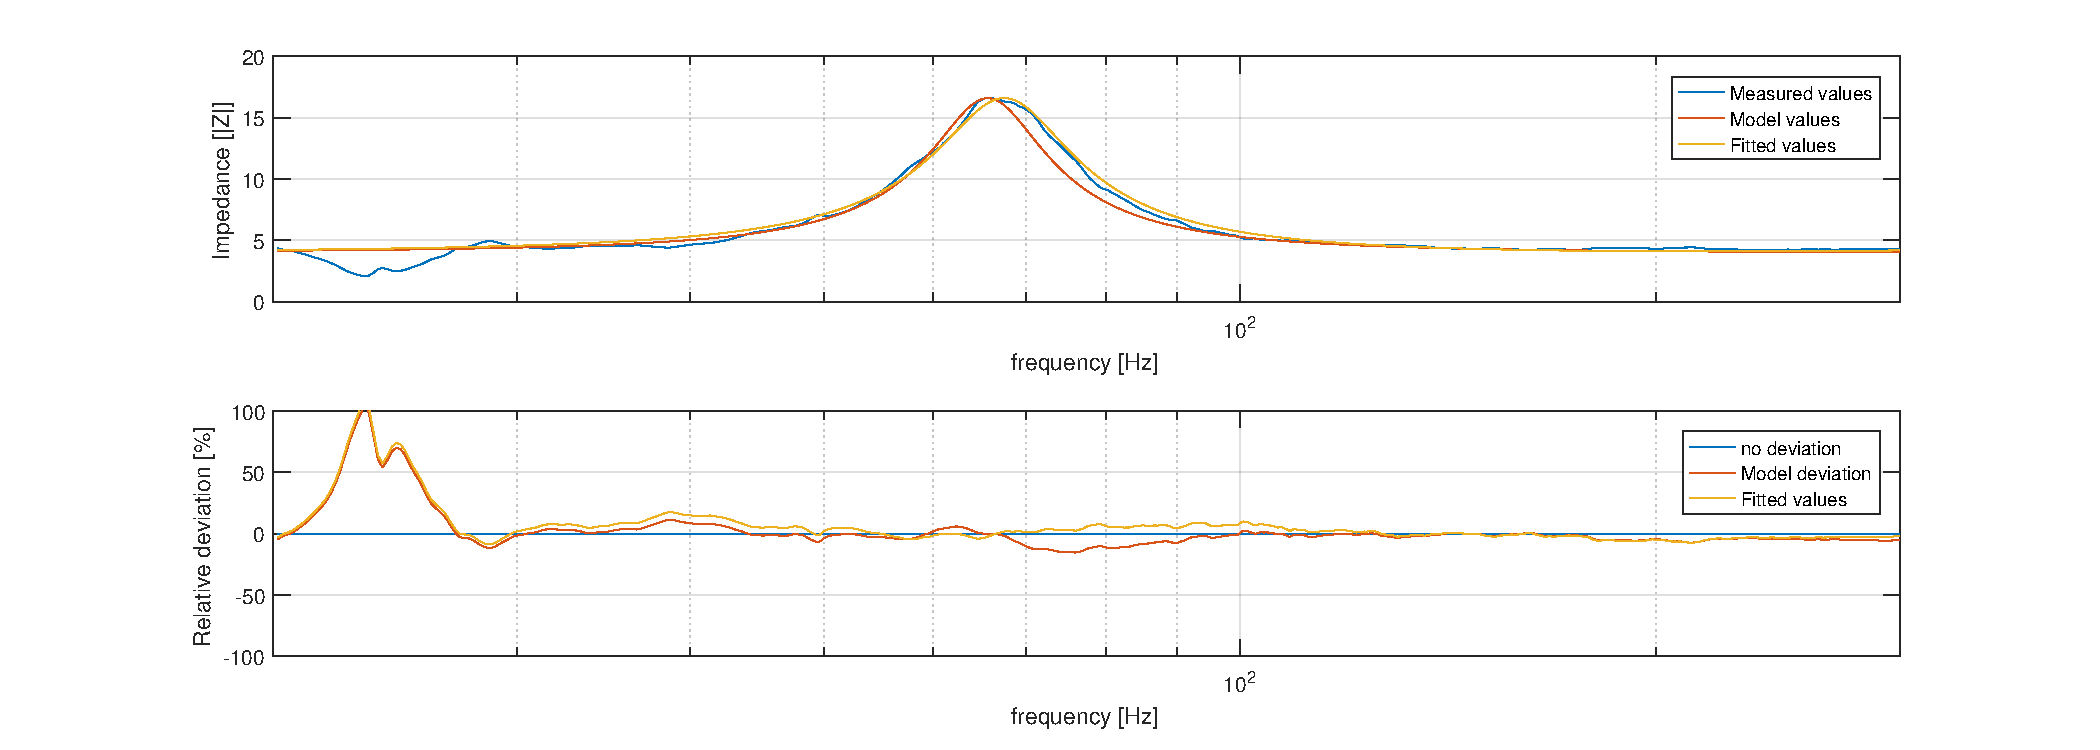
\includegraphics[height=0.2\paperheight]{Figures/Relative_Deviation_Bass_Impedance_Models}%
  }\par\medskip
\subcaptionbox{Relative deviations of the models for the mid speaker\label{fig:Relative_Deviation_Mid_Impedance_Models}}{%
  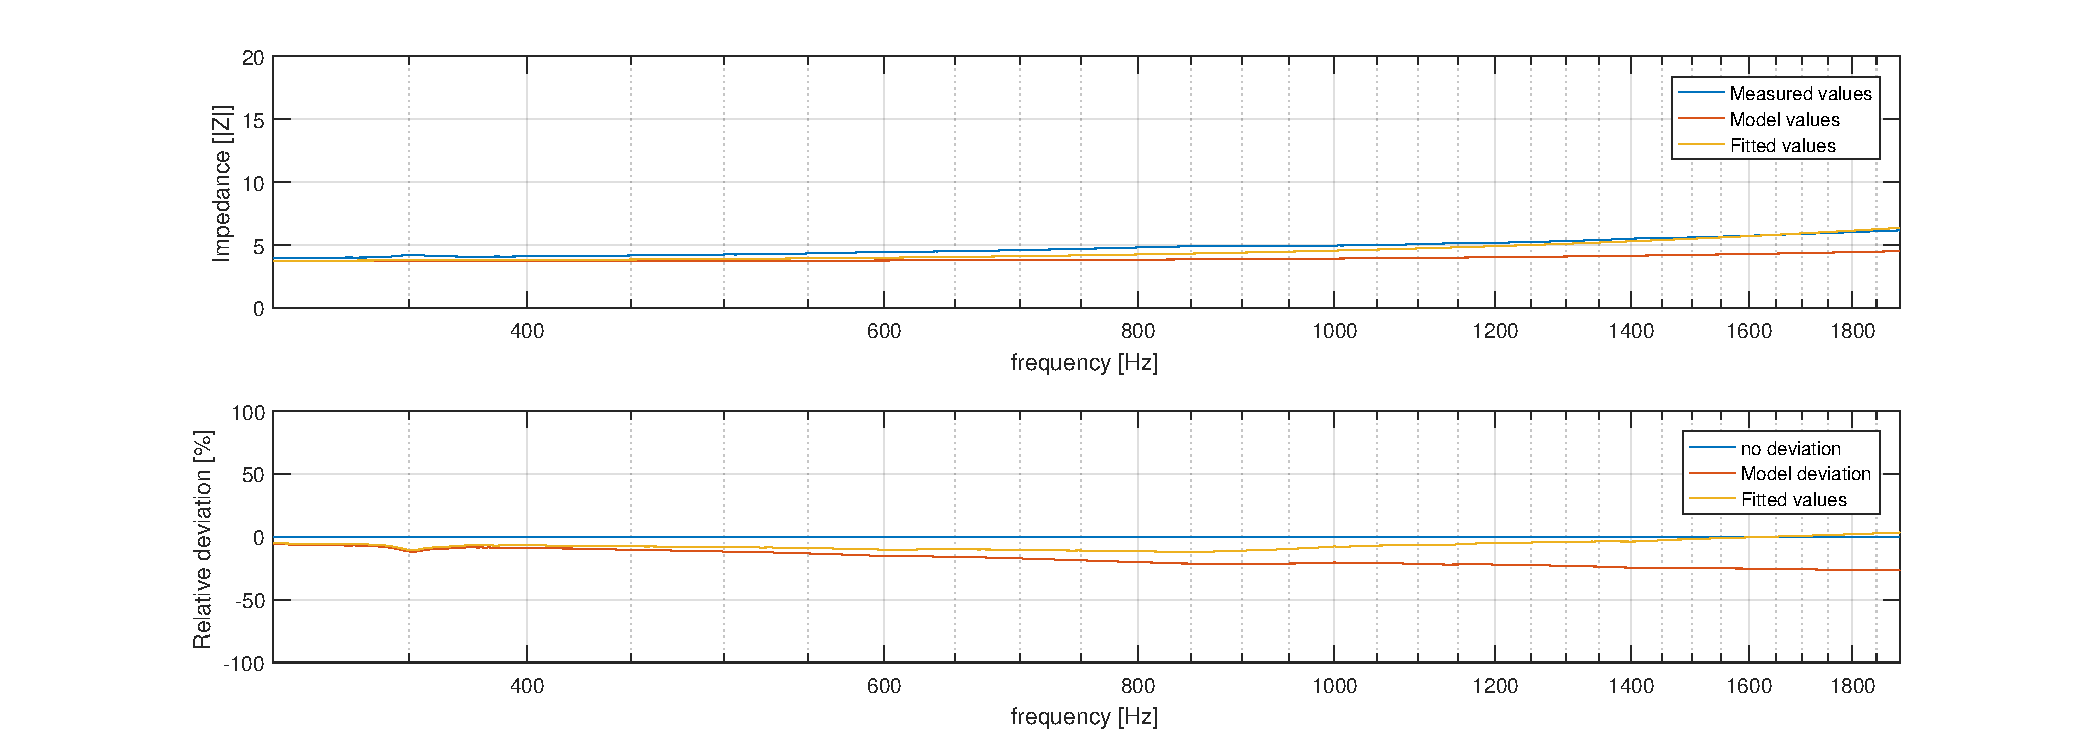
\includegraphics[height=0.2\paperheight]{Figures/Relative_Deviation_Mid_Impedance_Models}%
  }\par\medskip        
\subcaptionbox{Relative deviations of the models for the high speaker\label{fig:Relative_Deviation_High_Impedance_Models}}{%
  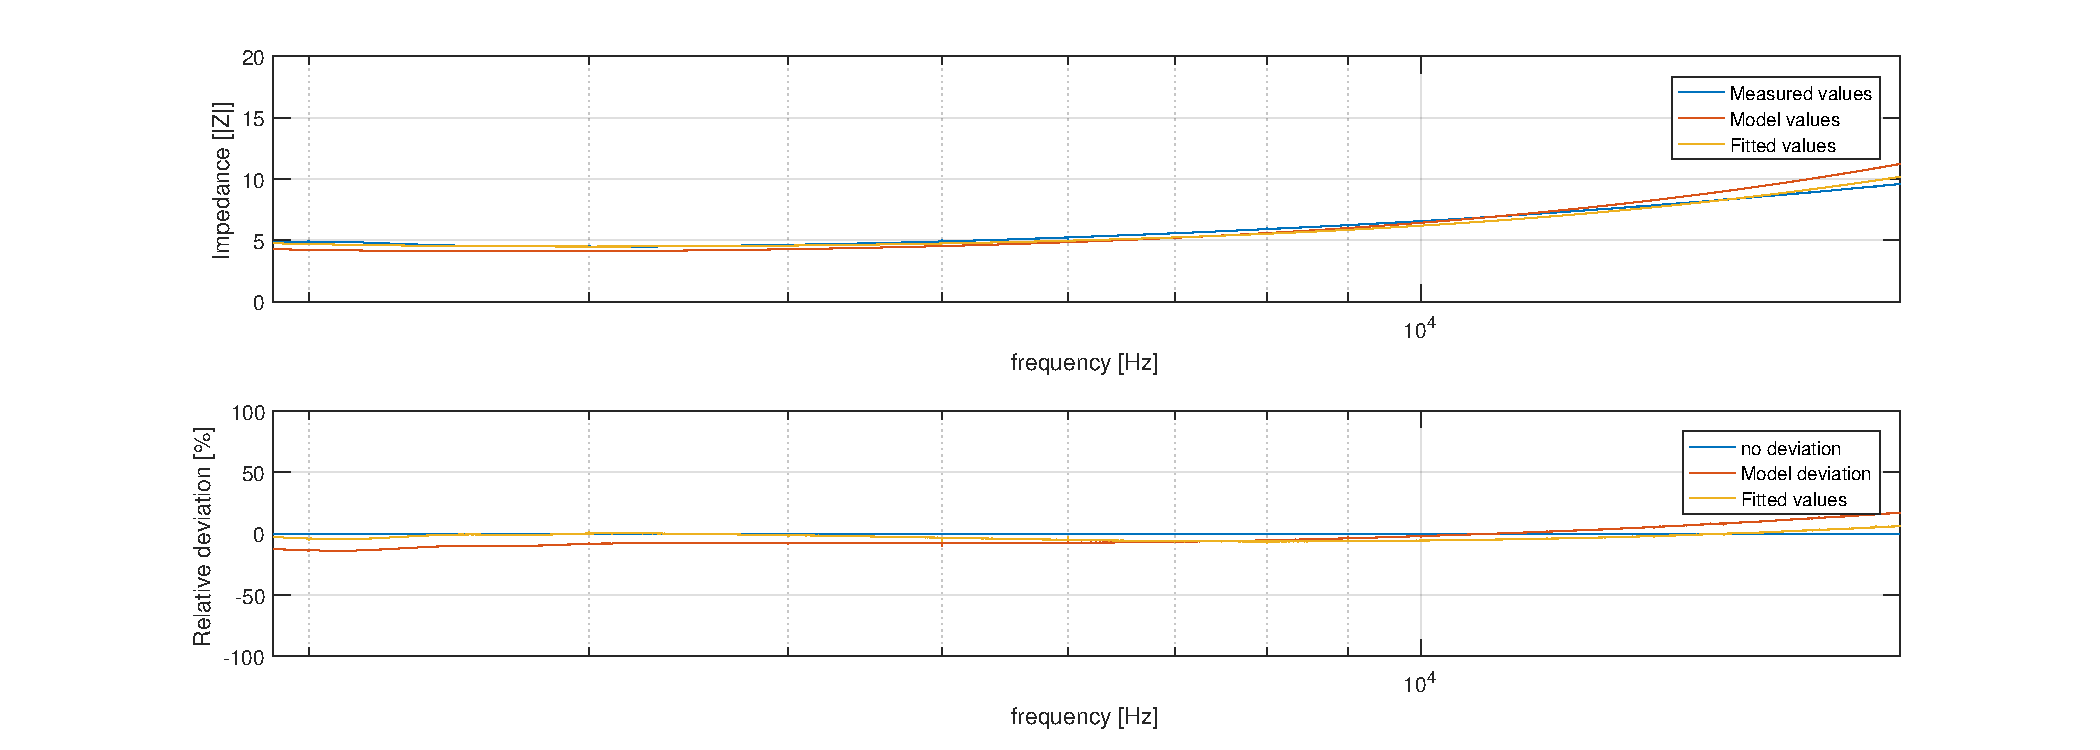
\includegraphics[height=0.2\paperheight]{Figures/Relative_Deviation_High_Impedance_Models}%
  }
\caption{Relative deviation of the different models with respect to the measured data.}
\label{fig:Calculated_impedance_models_fitted}
\end{figure}



\subsection{Phase shift of the speakers}
\begin{figure}[H]
\centering
\subcaptionbox{Phase shift of the high.  \label{fig:Tweeter_phaseshift_JBT}}{%
  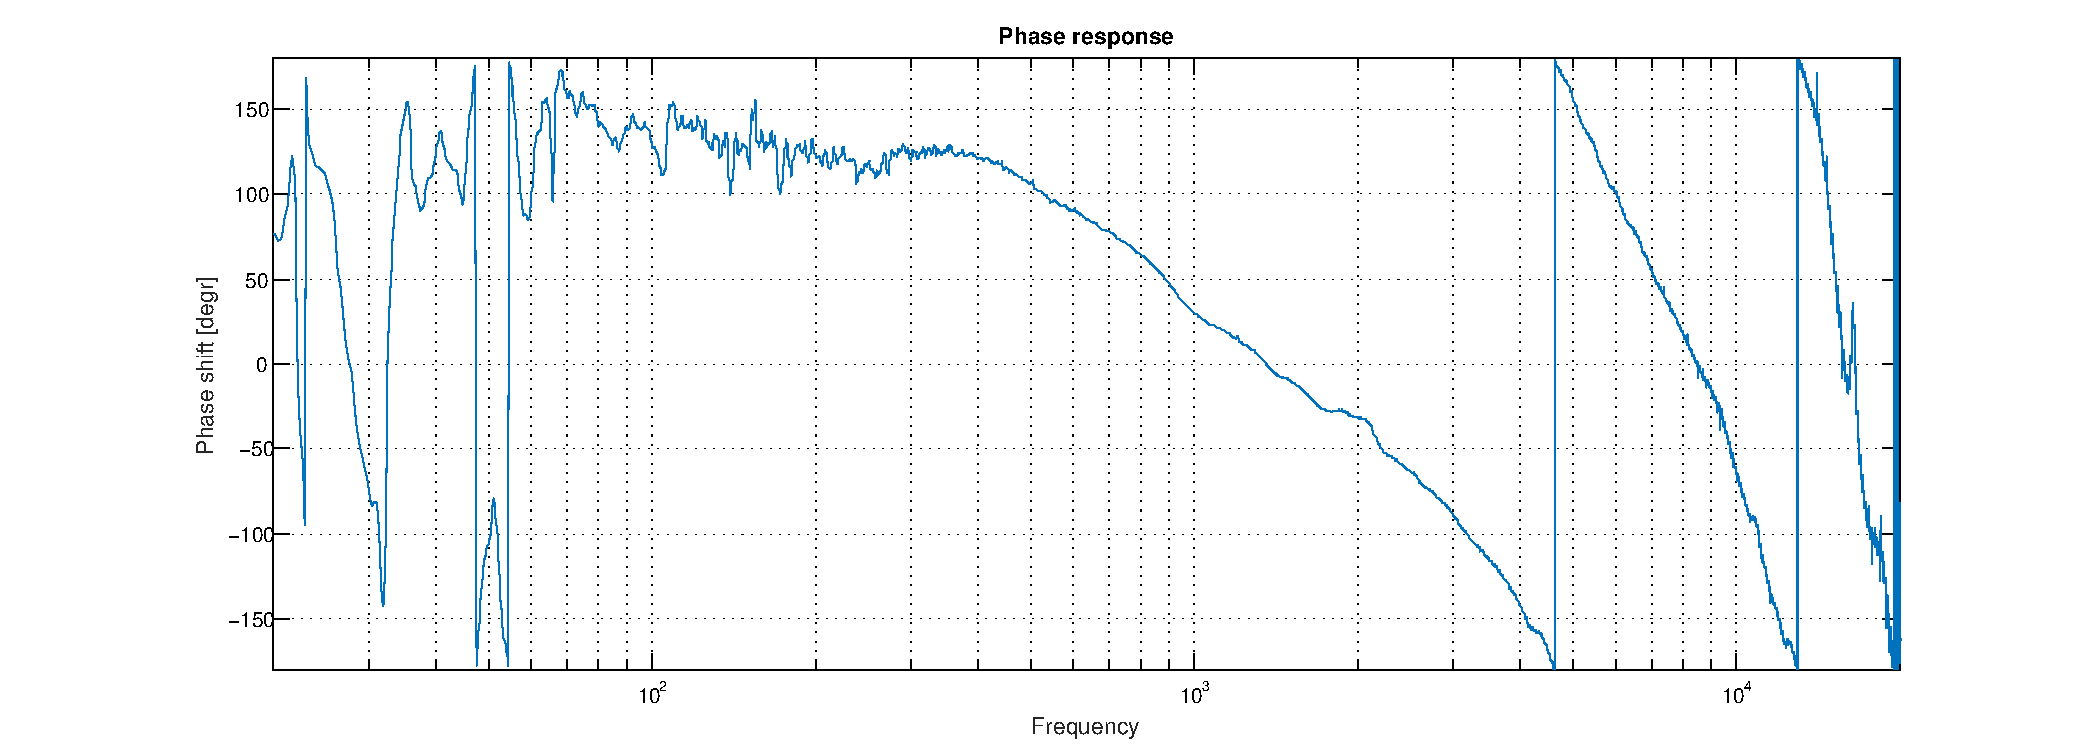
\includegraphics[height=0.2\paperheight]{Figures/Tweeter_phaseshift_JBT}%
  }\par\medskip
  
  \subcaptionbox{phase shift  of the woofer. \label{fig:Wooofers_phaseshift_JBT}}{%
  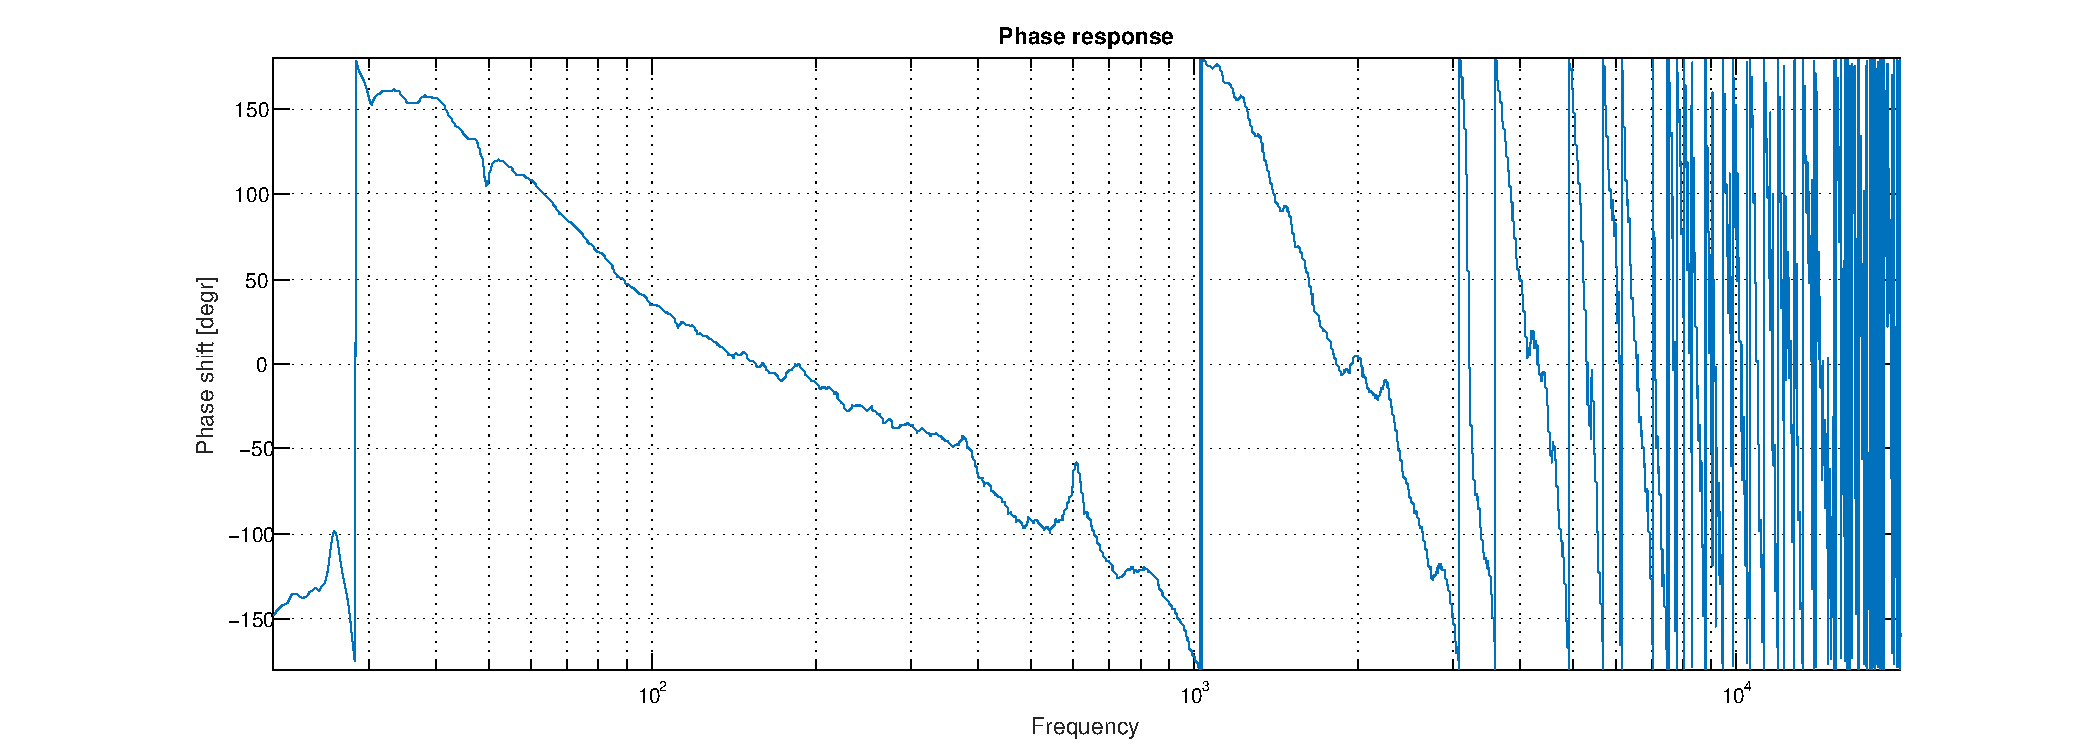
\includegraphics[height=0.2\paperheight]{Figures/Woofers_phaseshift_JBT}%
  }\par\medskip
  
\subcaptionbox{phase shift of the mid.  \label{fig:Mid_phaseshift_JBT}}{%
  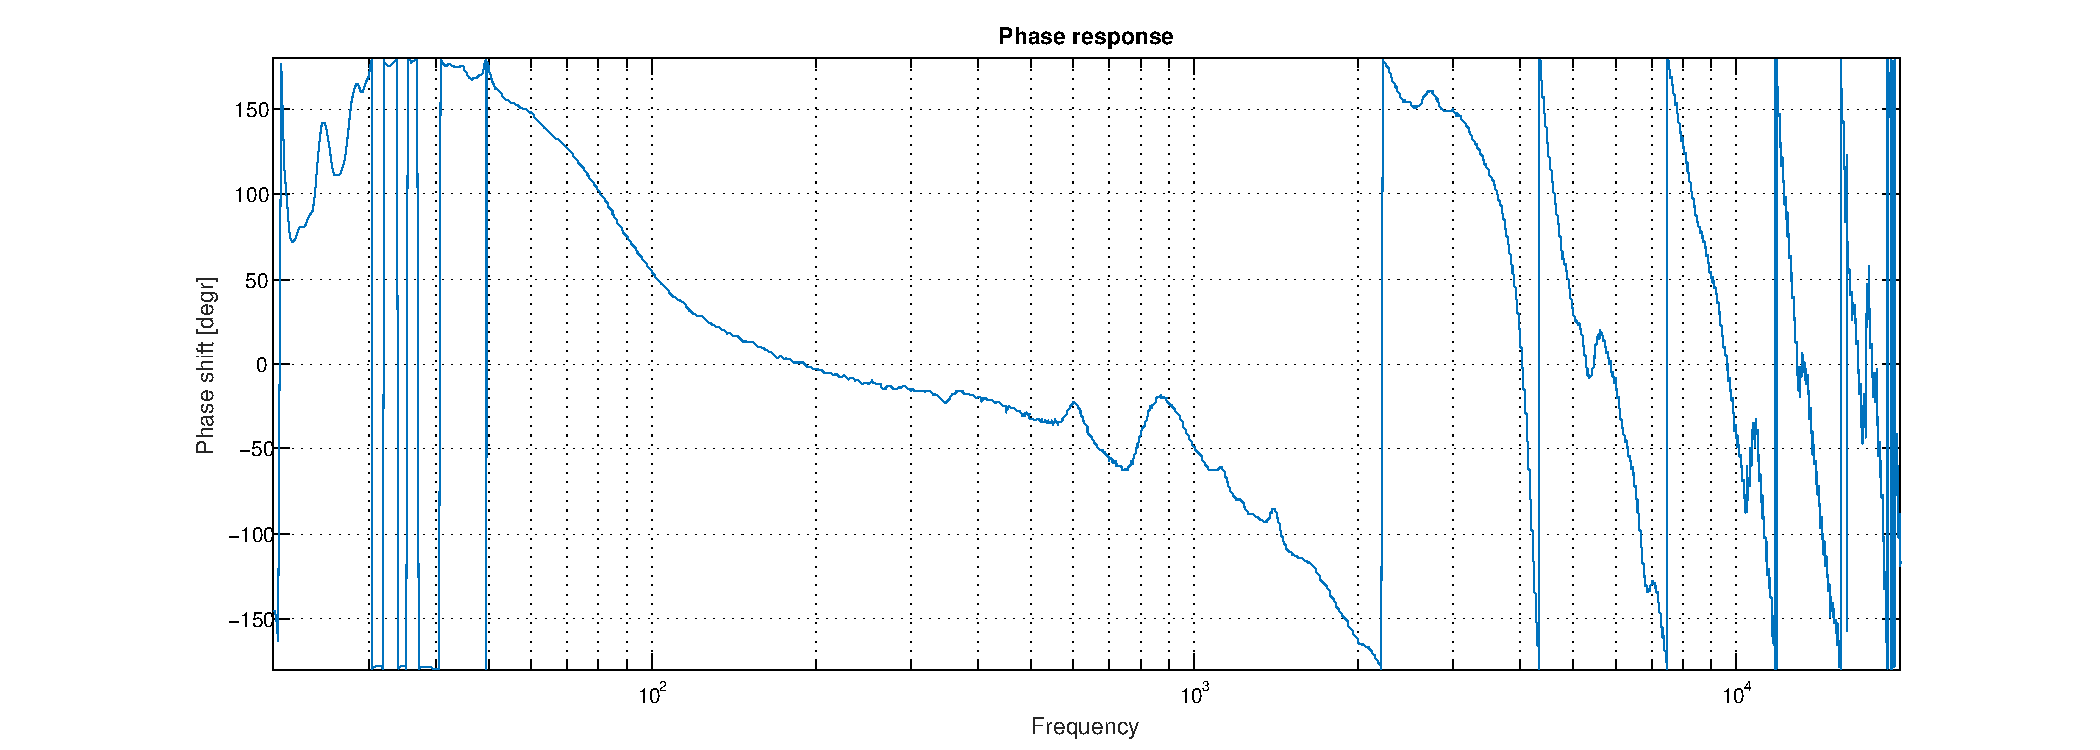
\includegraphics[height=0.2\paperheight]{Figures/Mid_phaseshift_JBT}%
  }
\caption{phase shift of the the speakers}
\label{fig:Calculated_impedance_models_fitted}
\end{figure}

\subsection{Frequency response}
\begin{figure}[H]
\centering
\subcaptionbox{Frequency response of the high.  \label{fig:Tweeter_Response_JBT}}{%
  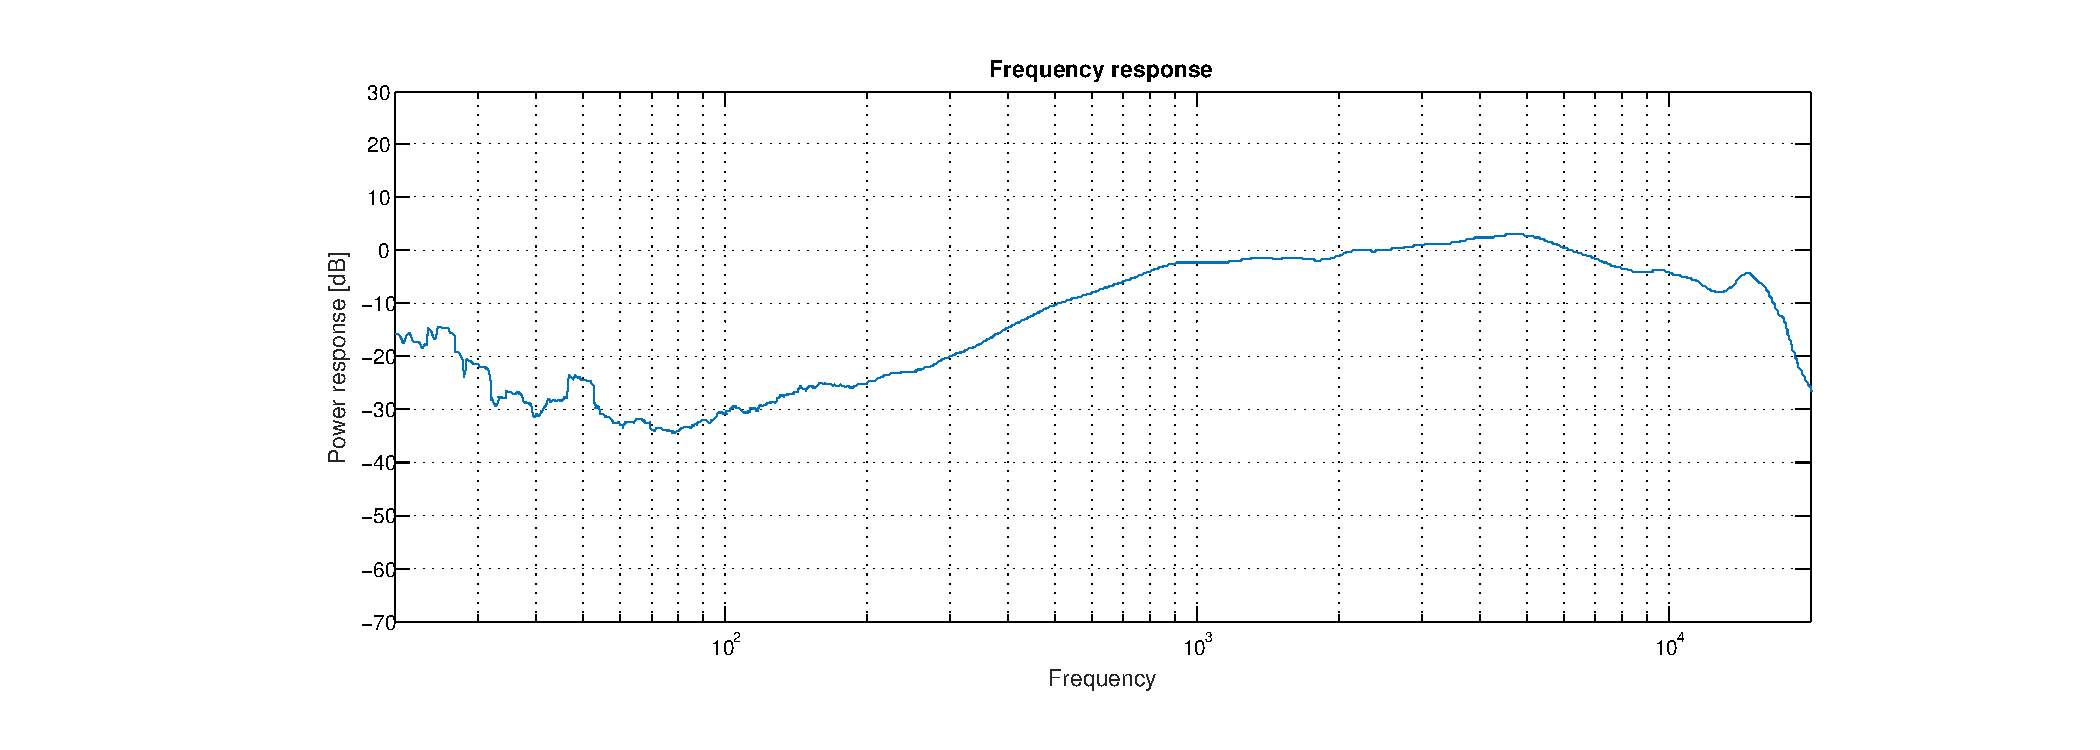
\includegraphics[height=0.2\paperheight]{Figures/Tweeter_Response_JBT}%
  }\par\medskip
  
  \subcaptionbox{Frequency response of the woofer \label{fig:Wooofers_Response_JBT}}{%
  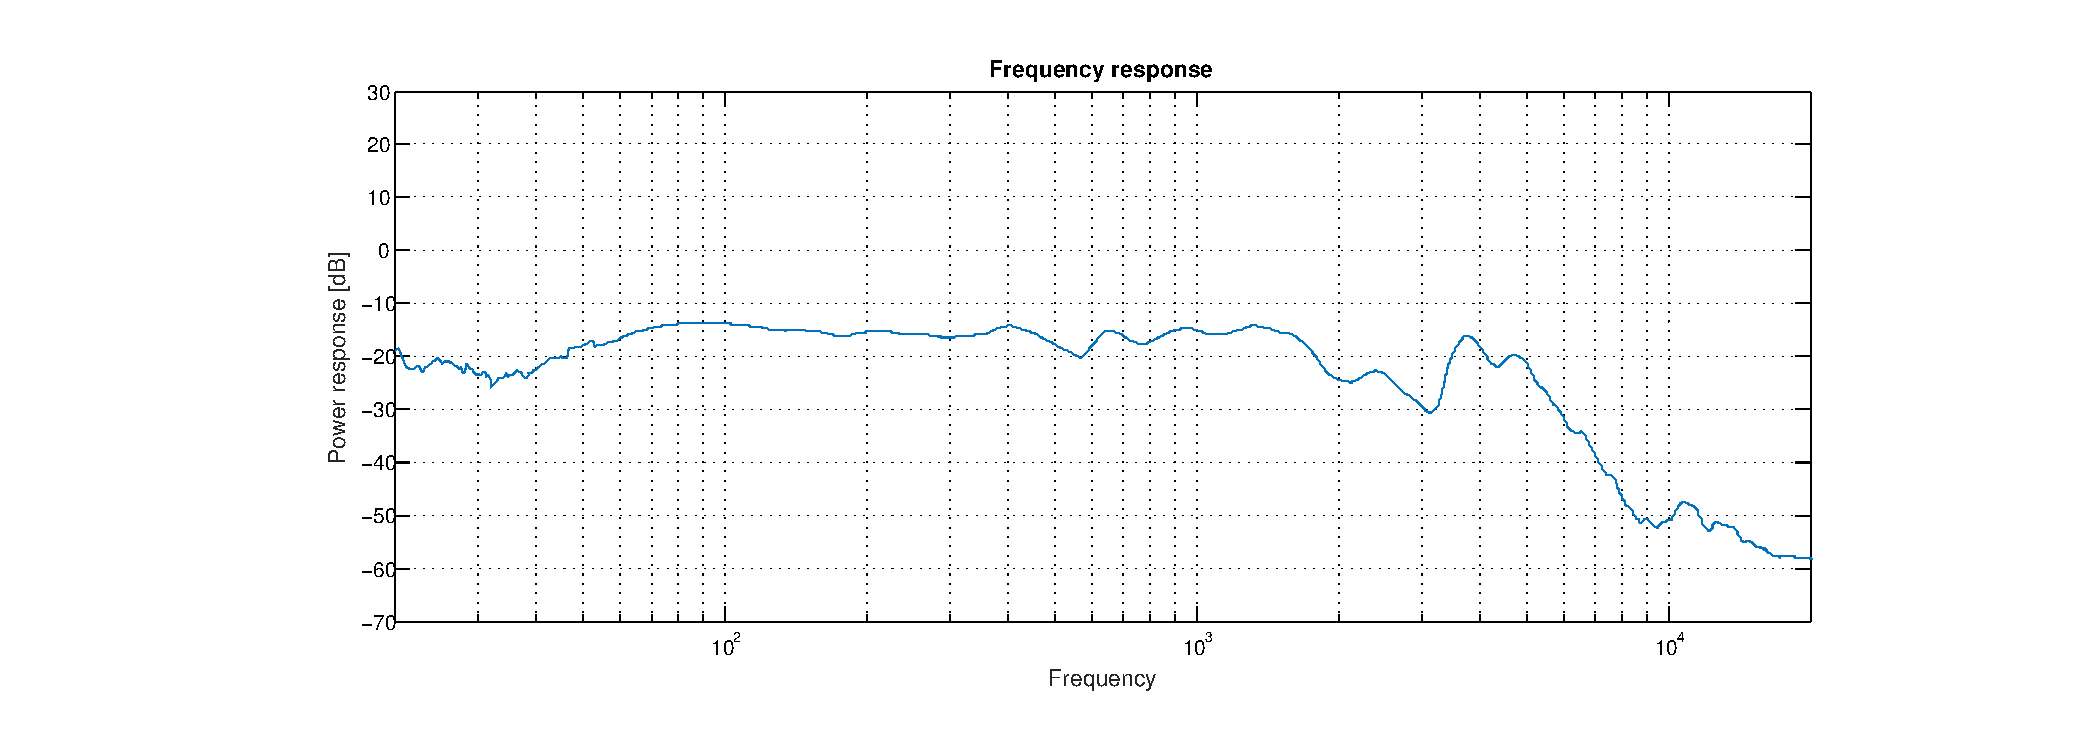
\includegraphics[height=0.2\paperheight]{Figures/Woofers_Response_JBT}%
  }\par\medskip
  
\subcaptionbox{Frequency response of the mid.  \label{fig:Mid_Response_JBT}}{%
  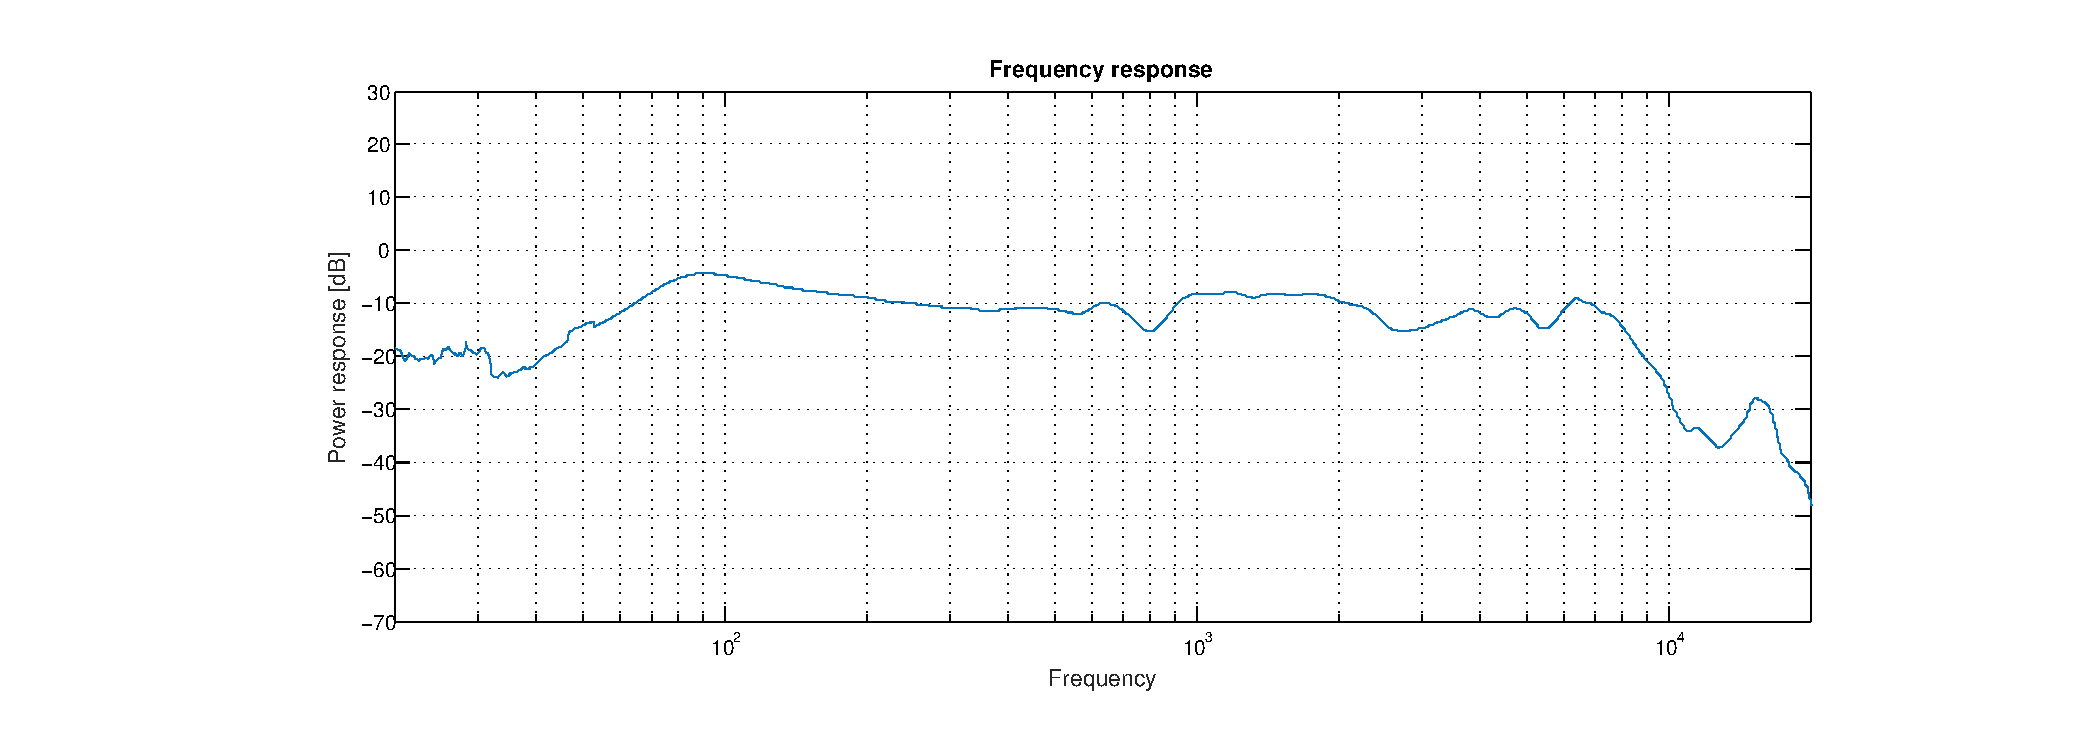
\includegraphics[height=0.2\paperheight]{Figures/Mid_Response_JBT}%
  }
\caption{Frequency response of the the speakers}
\label{fig:Calculated_impedance_models_fitted}
\end{figure}


\end{document}